\documentclass[onecolumn,10pt]{jhwhw}

\usepackage{epsfig} %% for loading postscript figures
\usepackage{amsmath}
\usepackage{graphicx}
\usepackage{caption}
\usepackage{subcaption}
\usepackage{grffile}
\usepackage{pdfpages}
\usepackage{algpseudocode}
\usepackage{wrapfig}
\usepackage{pgfplots}
\usepackage{amsfonts}
\usepackage{booktabs}
\usepackage{siunitx}
\usepackage{commath}
\usepackage{rotating}
\usepackage{url}
\usepackage{multimedia}
\usepackage{hyperref}
\usepackage{mathtools}
\usepackage{dirtytalk}

\usepackage{makecell}
\renewcommand\theadalign{cb}
\renewcommand\theadfont{\bfseries}
\renewcommand\theadgape{\Gape[4pt]}
\renewcommand\cellgape{\Gape[4pt]}

% Default fixed font does not support bold face
\DeclareFixedFont{\ttb}{T1}{txtt}{bx}{n}{12} % for bold
\DeclareFixedFont{\ttm}{T1}{txtt}{m}{n}{12}  % for normal

% Custom colors
\usepackage{color}
\usepackage{listings}
\usepackage{framed}
\usepackage{caption}
\usepackage{bm}
\captionsetup[lstlisting]{font={small,tt}}

\definecolor{mygreen}{rgb}{0,0.6,0}
\definecolor{mygray}{rgb}{0.5,0.5,0.5}
\definecolor{mymauve}{rgb}{0.58,0,0.82}

\lstset{ %
  backgroundcolor=\color{white},   % choose the background color; you must add \usepackage{color} or \usepackage{xcolor}
  basicstyle=\ttfamily\footnotesize, % the size of the fonts that are used for the code
  breakatwhitespace=false,         % sets if automatic breaks should only happen at whitespace
  breaklines=true,                 % sets automatic line breaking
  captionpos=b,                    % sets the caption-position to bottom
  commentstyle=\color{mygreen},    % comment style
  deletekeywords={...},            % if you want to delete keywords from the given language
  escapeinside={\%*}{*)},          % if you want to add LaTeX within your code
  extendedchars=true,              % lets you use non-ASCII characters; for 8-bits encodings only, does not work with UTF-8
  frame=single,                    % adds a frame around the code
  keepspaces=true,                 % keeps spaces in text, useful for keeping indentation of code (possibly needs columns=flexible)
  columns=flexible,
  keywordstyle=\color{blue},       % keyword style
  language=Python,                 % the language of the code
  morekeywords={*,...},            % if you want to add more keywords to the set
  numbers=left,                    % where to put the line-numbers; possible values are (none, left, right)
  numbersep=5pt,                   % how far the line-numbers are from the code
  numberstyle=\tiny\color{mygray}, % the style that is used for the line-numbers
  rulecolor=\color{black},         % if not set, the frame-color may be changed on line-breaks within not-black text (e.g. comments (green here))
  showspaces=false,                % show spaces everywhere adding particular underscores; it overrides 'showstringspaces'
  showstringspaces=false,          % underline spaces within strings only
  showtabs=false,                  % show tabs within strings adding particular underscores
  stepnumber=1,                    % the step between two line-numbers. If it's 1, each line will be numbered
  stringstyle=\color{mymauve},     % string literal style
  tabsize=4,                       % sets default tabsize to 2 spaces
}

\usepackage{etoolbox}
\renewcommand{\lstlistingname}{Diagram}% Listing -> Algorithm
\patchcmd{\thebibliography}{\chapter*}{\section*}{}{}

\usepackage[utf8]{inputenc}
\usepackage{fourier}
\usepackage{array}
\usepackage{makecell}

% \renewcommand\theadalign{cb}
% \renewcommand\theadfont{\bfseries}
% \renewcommand\theadgape{\Gape[1pt]}
% \renewcommand\cellgape{\Gape[1pt]}

\author{John Karasinski}
\title{HST Rendezvous}

\begin{document}
%\maketitle

\chapter{Introduction}

% \begin{figure}[h!]
% \begin{center}
% 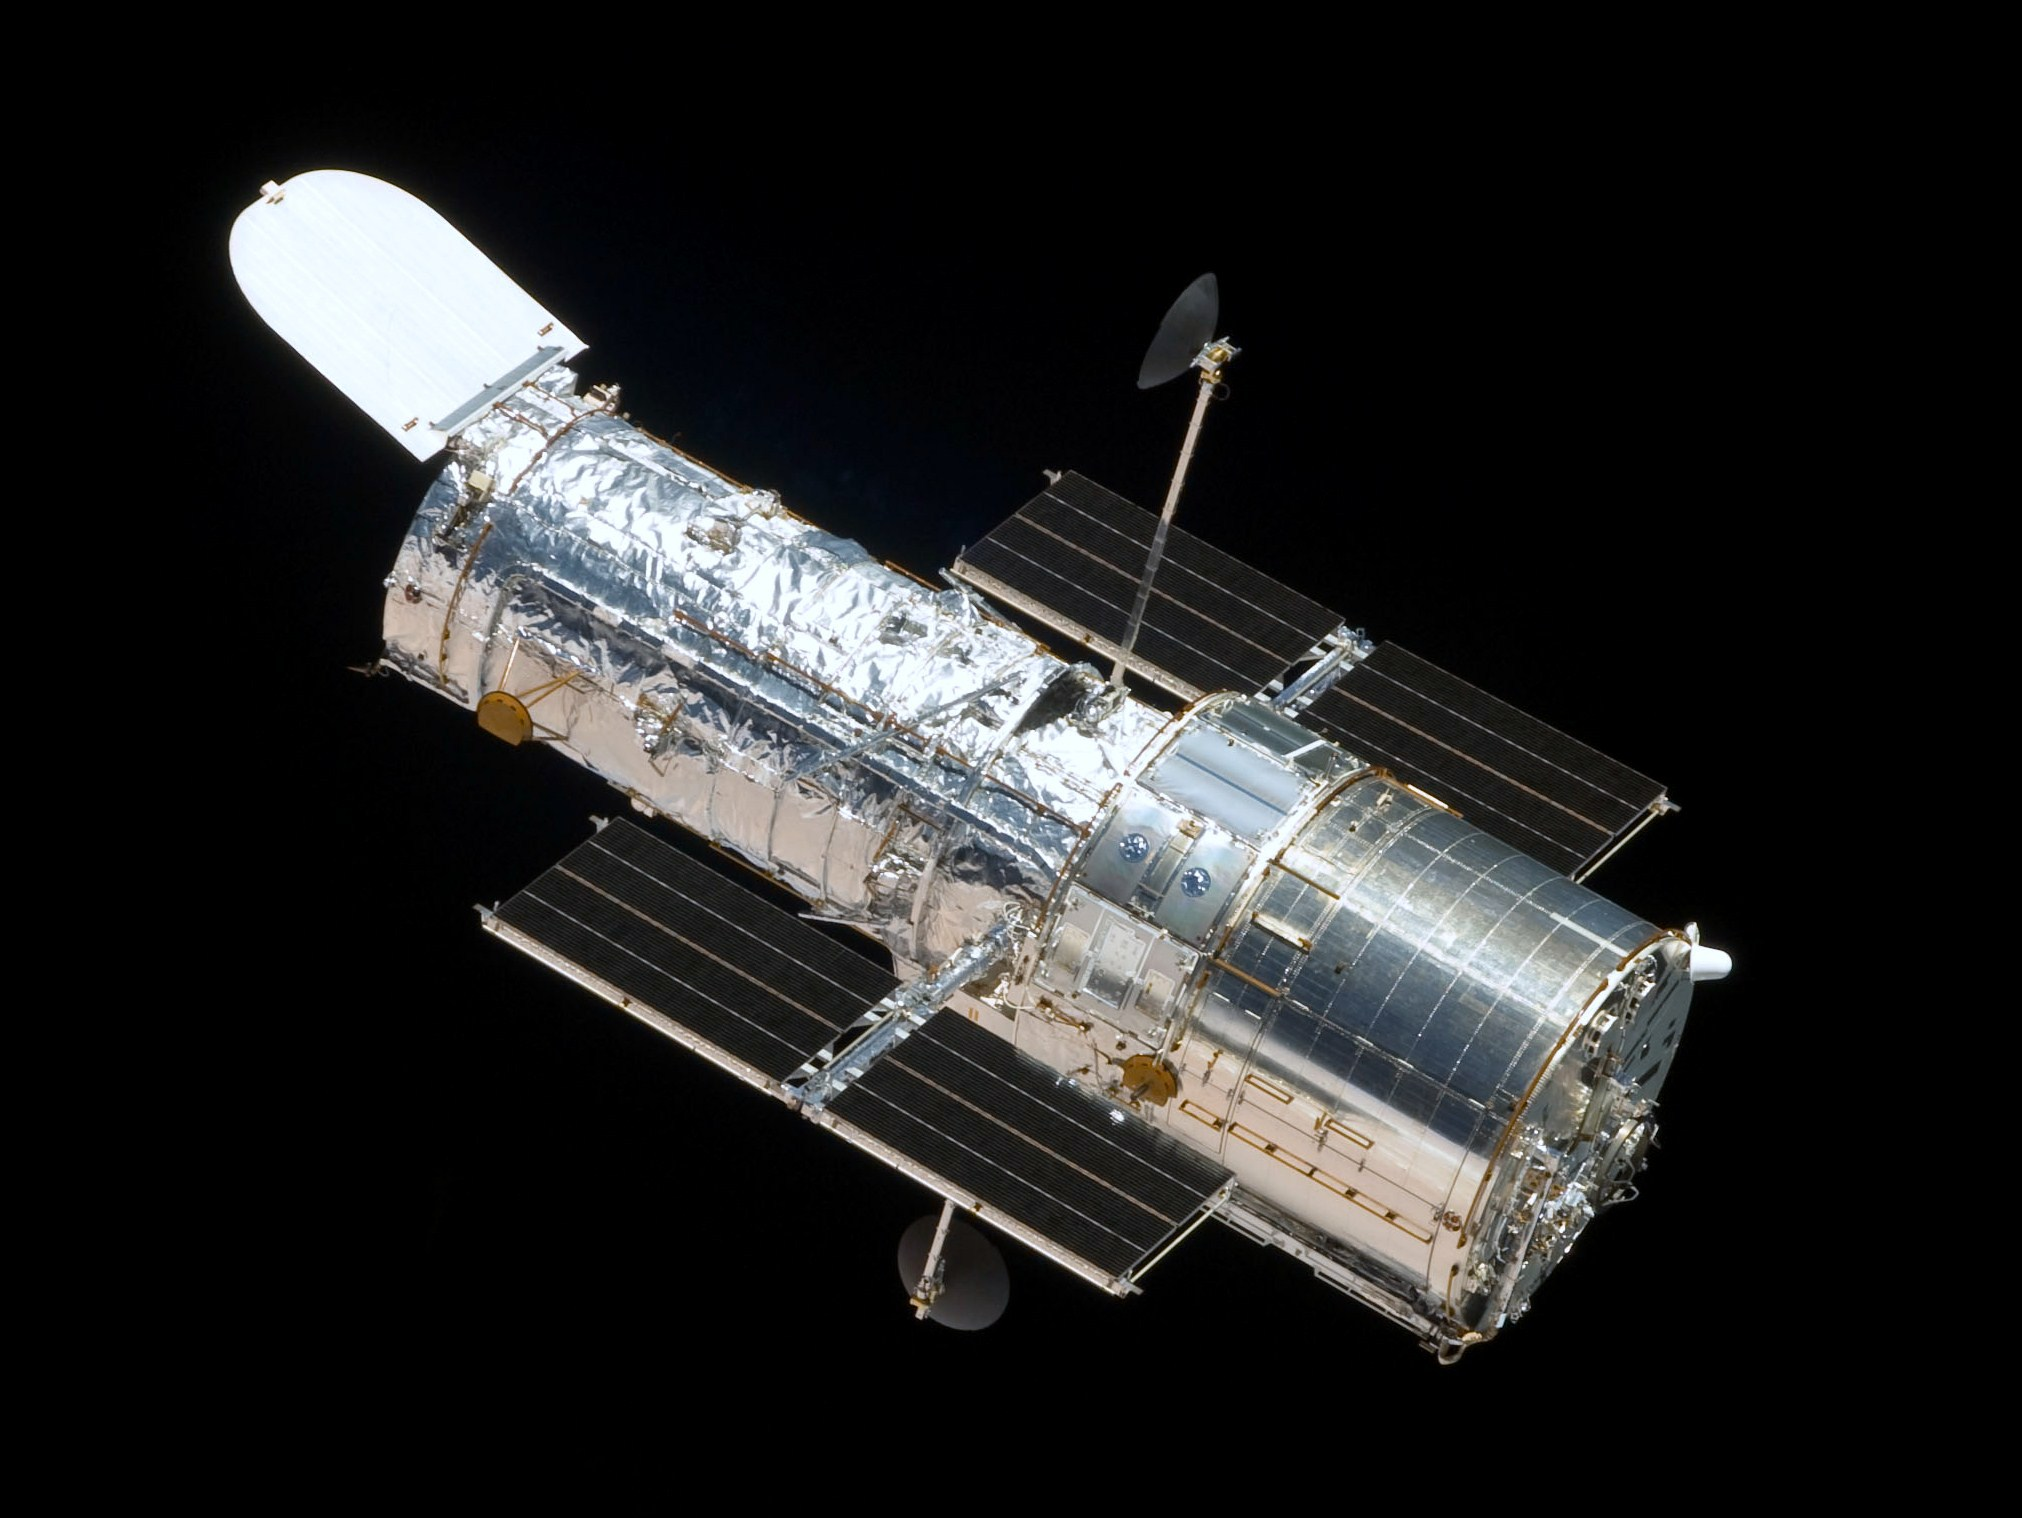
\includegraphics[width=1\textwidth]{imgs/HST-SM4.jpeg}
% \caption{The Hubble Space Telescope as seen from the departing Space Shuttle Atlantis, flying Servicing Mission 4 (STS-125), the fifth and final human spaceflight to it.}
% \label{fig:density}
% \end{center}
% \end{figure}

\begin{figure}[tbh]
\begin{center}
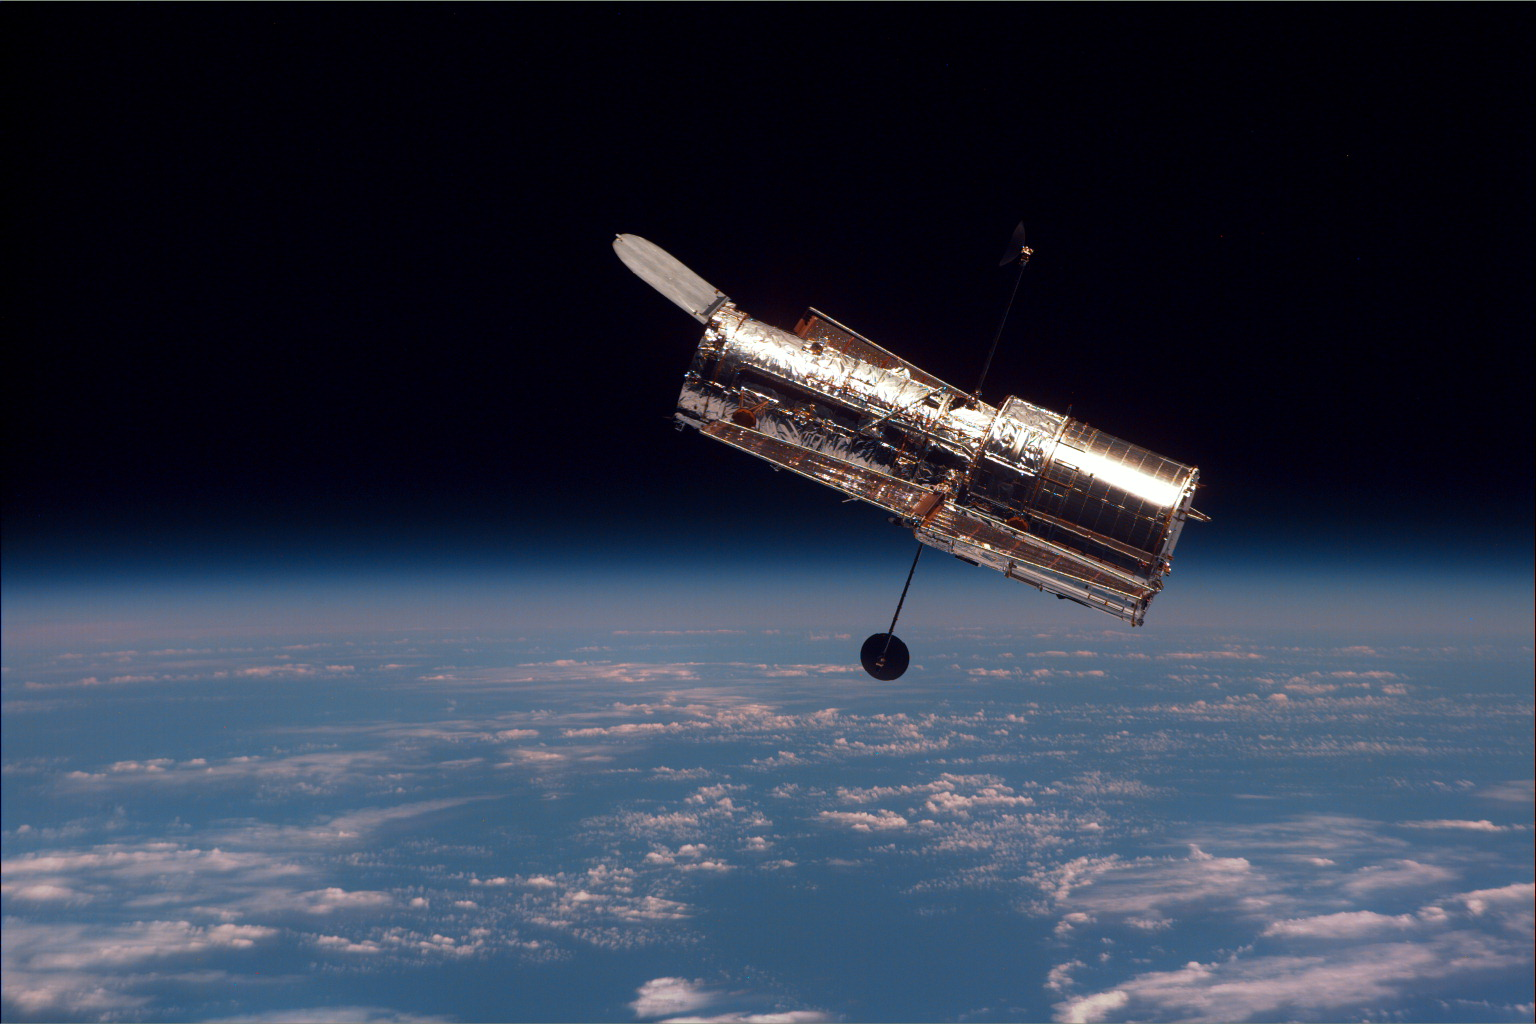
\includegraphics[width=1\textwidth]{imgs/hst.jpg}
\caption{This photograph of NASA's Hubble Space Telescope was taken on the second servicing mission to the observatory in 1997.}
\label{fig:density}
\end{center}
\end{figure}

\section{Mission Purpose}
The Hubble Reboost Vehicle (HRV) shall extend the Hubble Space Telescope's (HST) operational lifetime to 5 years beyond the James Webb Space Telescope's (JWST) October 2023 launch date. This will be achieved by reboosting HST into a circular orbit such that it's useful operation until orbit decay is extended to October of 2028.

\section{Mission Timeline}
The mission to re-boost the HST will be composed of multiple phases, as described in the table below. The entire duration of the mission will be no longer than 60 hours.

\begin{table}[h!]
\begin{center}
\begin{tabular}{l r}
\toprule
Mission Phase & Duration (hours) \\
\midrule
1. Launch (delivered to parking orbit) & 0.27 \\
2. Maintain parking orbit for necessary phasing time & up to 24 \\
3. Transfer to HST altitude & 1.53 \\
4. Rendezvous and dock with the HST &  \\
5. Boost HST to new orbit & 1.60 \\
6. Undock and separate from HST &  \\
7. Maintain orbit for necessary phasing time & up to 24 \\
8. De-orbit to burn up in the atmosphere & 0.77 \\
\bottomrule
Max time: & 52.17 \\
\bottomrule
\end{tabular}
\end{center}
% \caption{}
% \label{properties}
\end{table}

A launch date (September 2019) was chosen to provide the most direct route to the HST. By launching when the HST is directly over the launch site (Kennedy Space Center), the re-boost vehicle will match its inclination and longitude of ascending node. This prevents the need for any costly plane changes.

\section{Stakeholders}

% \begin{figure}[t!]
%     \centering
%     \begin{subfigure}[b]{0.4\textwidth}
%         \includegraphics[width=\textwidth]{imgs/xtreme_deep_field.png}
%     \end{subfigure}
%     ~ %add desired spacing between images, e. g. ~, \quad, \qquad, \hfill etc.
%     %(or a blank line to force the subfigure onto a new line)
%      \begin{subfigure}[b]{0.4\textwidth}
%         \includegraphics[width=\textwidth]{imgs/Pillars_of_creation_2014_HST_WFC3_medium_res.jpg}
%     \end{subfigure}
%     ~ %add desired spacing between images, e. g. ~, \quad, \qquad, \hfill etc.
%       %(or a blank line to force the subfigure onto a new line)
%     \begin{subfigure}[b]{0.4\textwidth}
%         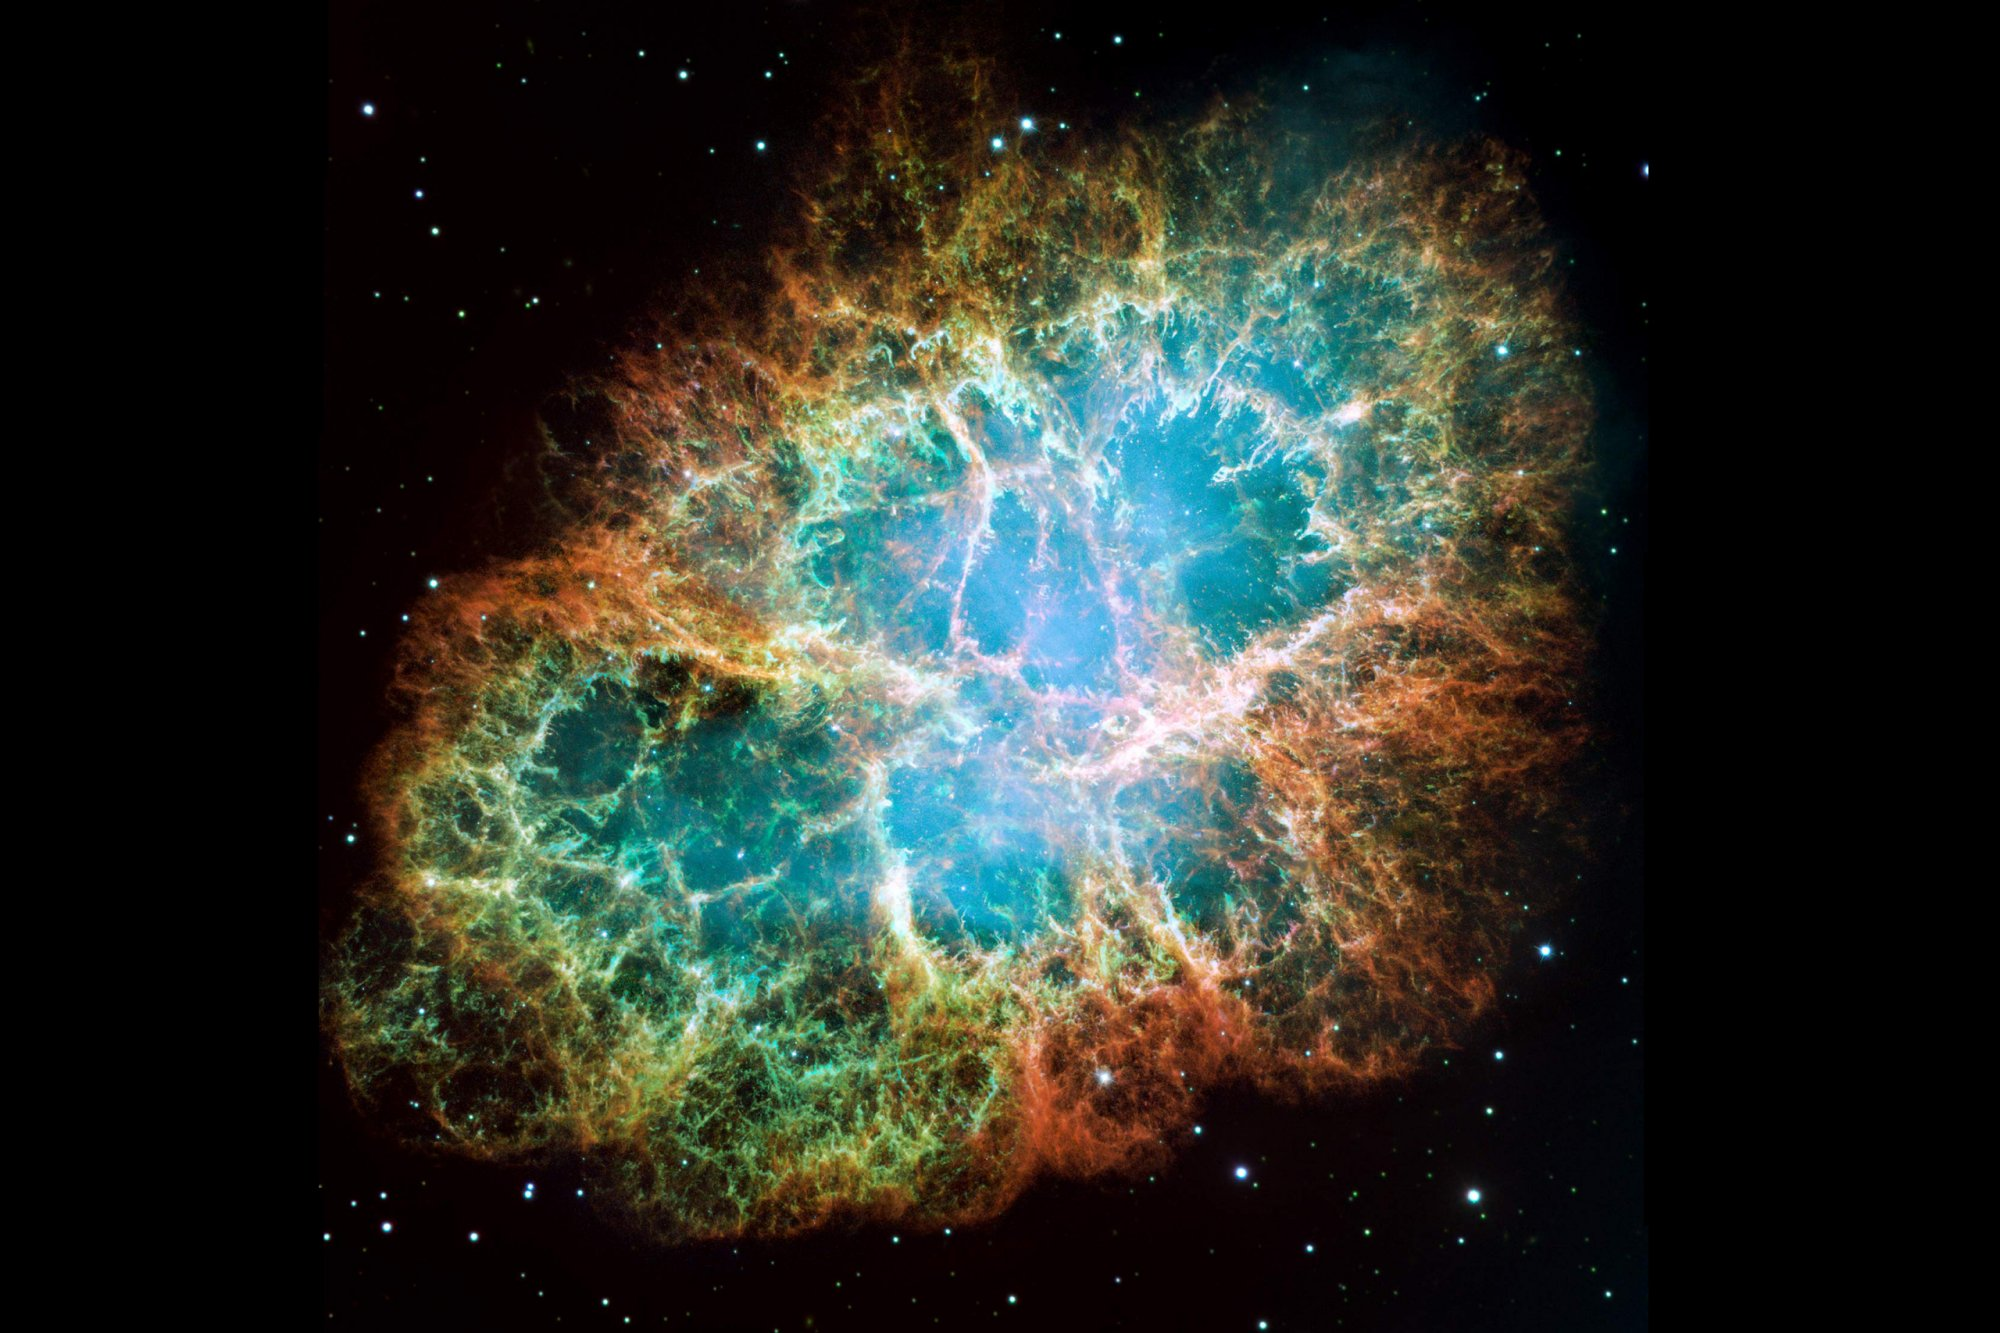
\includegraphics[width=\textwidth]{imgs/crab.jpg}
%     \end{subfigure}
%     ~ %add desired spacing between images, e. g. ~, \quad, \qquad, \hfill etc.
%     %(or a blank line to force the subfigure onto a new line)
%     \begin{subfigure}[b]{0.4\textwidth}
%         \includegraphics[width=\textwidth]{imgs/M104_ngc4594_sombrero_galaxy_hi-res.jpg}
%     \end{subfigure}
%     \caption{Hubble has taken many photos of iconic space objects, including the Hubble Extreme Deep Field, Pillars of Creation, the Crab Nebulae, and the Sombrero Galaxy.}
%     \label{fig:animals}
% \end{figure}

Hubble has a large number of stakeholders. Since it's launch in 1990, the Hubble Space Telescope has acted as one of the most vital research tools for astronomy, and over 9,000 papers based on Hubble data have been published in peer-reviewed journals. Hubble has made a large number of important discoveries, leading to significant changes in how we think about the universe. Among its primary mission targets was to measure distances to Cepheid variable stars more accurately than ever before. Accurate measurement of the Cepheid variable constrains the value of the Hubble constant, the measure of the rate at which the universe is expanding, which has allowed scientists to very accurately calculate the age of the universe.

Hubble has also been extremely successful in generating public relations, both due to its scientific achievements and the wealth of memorable images it has produced. The public is extremely invested in Hubble, both from their large contributions to its construction and operational costs. Aside from Hubble's scientific goals, it also helps fulfill two of NASA's key agency objectives to:
\begin{itemize}
\setlength\itemsep{0em}
\item Improve science literacy by engaging the public in NASA missions and discoveries, and their benefits, through such avenues as public programming, community outreach, mass media, and the Internet.
\item Increase public awareness and understanding of how research and innovations in aerospace technology affect and improve the quality of life.
\end{itemize}

The HST was built by the United States space agency NASA, with contributions from the European Space Agency (ESA). The Space Telescope Science Institute (STScI) selects Hubble's targets and processes the resulting data, while the Goddard Space Flight Center controls the spacecraft~\footnote{"Hubble Essentials". Hubblesite.org. Retrieved March 3, 2016.}. As such, NASA, ESA, STScI, and NASA Goddard are among the chief stakeholders in a robotic reboost mission. Other organizations that have constructed and worked with HST, such as JPL and ITT, would obviously be affected by our interacting with HST. An incomplete list of stakeholders is
\begin{itemize}
\setlength\itemsep{0em}
\item NASA Headquarters (HQ)
\item NASA Goddard Space Flight Center (GSFC)
\item The European Space Agency (ESA)
\item The Space Telescope Science Institute (STScI)
\item The Jet Propulsion Laboratory (JPL)
\item ITT (formerly Kodak)
\item International universities and space agencies
\item The National Reconnaissance Office (NRO)
\item Department of Defense (DoD)
\item Other governmental organizations
\item The public
\end{itemize}

While none of the stakeholders involved in the Hubble project would necessarily mind extending the project for several years, damaging Hubble would be much worse than leaving it in it's current orbit. As such, the primary goal of the HRV is to do no harm to Hubble. The mission can succeed only if we can it can be accomplished within the stakeholders' limits of acceptable risk.

% \section{Concept of Operations}

% \subsection{Communication}
% Chris will write these sections.

% \subsection{What's ground control doing}
% The Hubble Repair Vehicle (HRV) will act as a primarily automatic vehicle. Despite this, ground control will be in continuous contact with the HRV throughout the lifetime of the mission, and will have the option of delaying or aborting orbital transfers and docking and rendezvous maneuvers. Before each orbital maneuver, ground control will



% After being dropped off from the launch vehicle, HRV will communicate with ground operations. After a brief instrument and spacecraft health check, HRV will receive updated HST state information, and updated orbital rendezvous parameters. Once this information is transferred, HRV will transfer to a higher orbit. HRV will be in contact during the phasing stage of the mission, and will wait at a holding point 15 km behind HST before entering the closing phase.

% \subsection{How's it going to be used?}

\section{Concept of Operations}
HRV mission control will be performed from NASA's Goddard Space Flight Center (GSFC). The site was chosen in order to incorporate several members of the HST team into the HRV team. Communication to both the HRV and HST will be performed primarily through the White Sands Complex and existing Tracking and Data Relay Satellite System (TDRSS). NASA's Kennedy Space Center (KSC) was selected as the launch site in order to launch into HST's orbit.

Upon launch the craft will be under the control of the United Launch Alliance (ULA). Telemetry will be monitored by the GSFC ground crew but control will not be handed over until the payload fairing separation. Upon being ejected from the payload, any primary systems not running start up. The HRV “wakes up” and starts to determine its attitude and position. During this time GSFC is also making attempts for their first radio acquisition. With the system fully booted and telemetry coming in, the HRV can start its mission.

The first step of the mission is to increase the HRV orbit out of the parking orbit. This requires a large burn to transfer to an orbit closer to HST then another burn to circularize. Any mission critical operation such as this requires confirmation from the ground crew. HRV telemetry and the calculated burn are relayed to the ground crew. The ground crew confirms the information and gives the HRV the go ahead to perform the burn. Any time the HRV is waiting for a critical response, a timer is also started. If an extended period of time passes without a command then end of mission deorbit procedures are started.

After circularizing to an orbit below HST, the rendezvous starts. The HRV is allowed to phase towards the HST until starting the final approach. The final approach is performed in two stages depending on the distance from the target. At this point the HST starts relaying telemetry directly to HRV through the low gain antennas. In the last moments of docking the craft is given more autonomy. There is no time to check every correction therefore a standard manual abort/override is built into the system.

Once the berthing has taken place, the HST's attitude control system is used to repoint the pair of craft for a prograde burn. HRV performs the burn to increase the craft's orbit. HST rotates the pair of craft for a retrograde burn. HRV performs a burn to circularize into the final target orbit. All of these are critical operations requiring the ground crew to confirm any actions.

With the main goal of the mission done, HRV detaches and separates to a safe distance. Once a sufficient distance is achieved from HST a final large burn is performed to deorbit the HRV. Before this burn is performed the final entry point is recalculated to ensure entry over the Pacific Ocean.

\chapter{Requirements}
\section{Customer Requirements}

The mission of the Hubble Reboost Vehicle (HRV) is to

\say{Reboost HST spacecraft to circular orbit so that useful operation until orbit decay is extended to 5 years beyond the JWST 10/23 launch date, i.e. to 10/28.} \\
\\
Thirteen requirements of the vehicle are taken directly from the Mission Requirements. To this end, the HRV must
\begin{enumerate}
\item Launch on an existing US launcher from Cape Canaveral into the HST orbit
\item Rendezvous and dock with HST
\item Use HST or rebooster ADCS to orient combined spacecraft for reboost
\item Reboost thrust must result in solar array boom deflection of no more than 50 cm
\item Undock from HST and destructively de-orbit into atmosphere
\item Send and receive state-vector, attitude, and system health telemetry to/from HST
\item Send and receive state-vector, attitude, and system health telemetry to/from NASA Mission Control Center (MCC), either directly, or indirectly via HST and or TDRS satellites
\item Be able to recover from one Single Event Upset per hour in the onboard Command and Control Computer
\item No requirement on duration of mission
\item Power and thermal requirements not specified --- to be determined by design to meet mission objectives
\item Main body of spacecraft bus must include MMOD shielding
\item ADCS must be able to recover from/override both jet-fail-on, and jet-fail cases during proximity operations without collision of mission failure
\item Loss of communications between rebooster and HST or MCC must not result in collision
\end{enumerate}

\section{Technical Requirements}

\subsection{Delta V Requirements}
The delta V requirements depend largely on the magnitude of the orbital maneuvers required. Therefore, it was necessary to first estimate where the HST will be both at the start of the mission (01/2020), and where it will be 8 1/2 years after the re-boost, i.e. what altitude is sufficient to extend the HST lifetime to 10/2028. Neither of these can be known precisely, but the latter in particular is subject to a high degree of uncertainty.

To determine where the HST will be, it was necessary to study where it has been. Two Line Element (TLE) data (requested and downloaded from \url{http://www.celestrak.com/}) provided a history of orbital parameters, from the launch date (April 24, 1990) to the present (February 6, 2016). This time period includes multiple past servicing missions, some of which included small re-boosts.

The parameter of greatest interest to the mission was the mean altitude (h) over time. This was calculated by using the mean motion (n), converted from revs/day to rad/s, to find the semi-major axis (a) of the ellipse:
\begin{align*}
h = a - r = \sqrt[3]{mu/n^2} - r
\end{align*}
where $\mu = \mu_{earth} = 398,600.4418$ x 10$^9$ m$^3$/s$^2$ and $r = r_{earth} = 6,378,136.49$ m. The result is shown in Figure~\ref{fig:fig1} below.

\begin{figure}[tb!]
\begin{center}
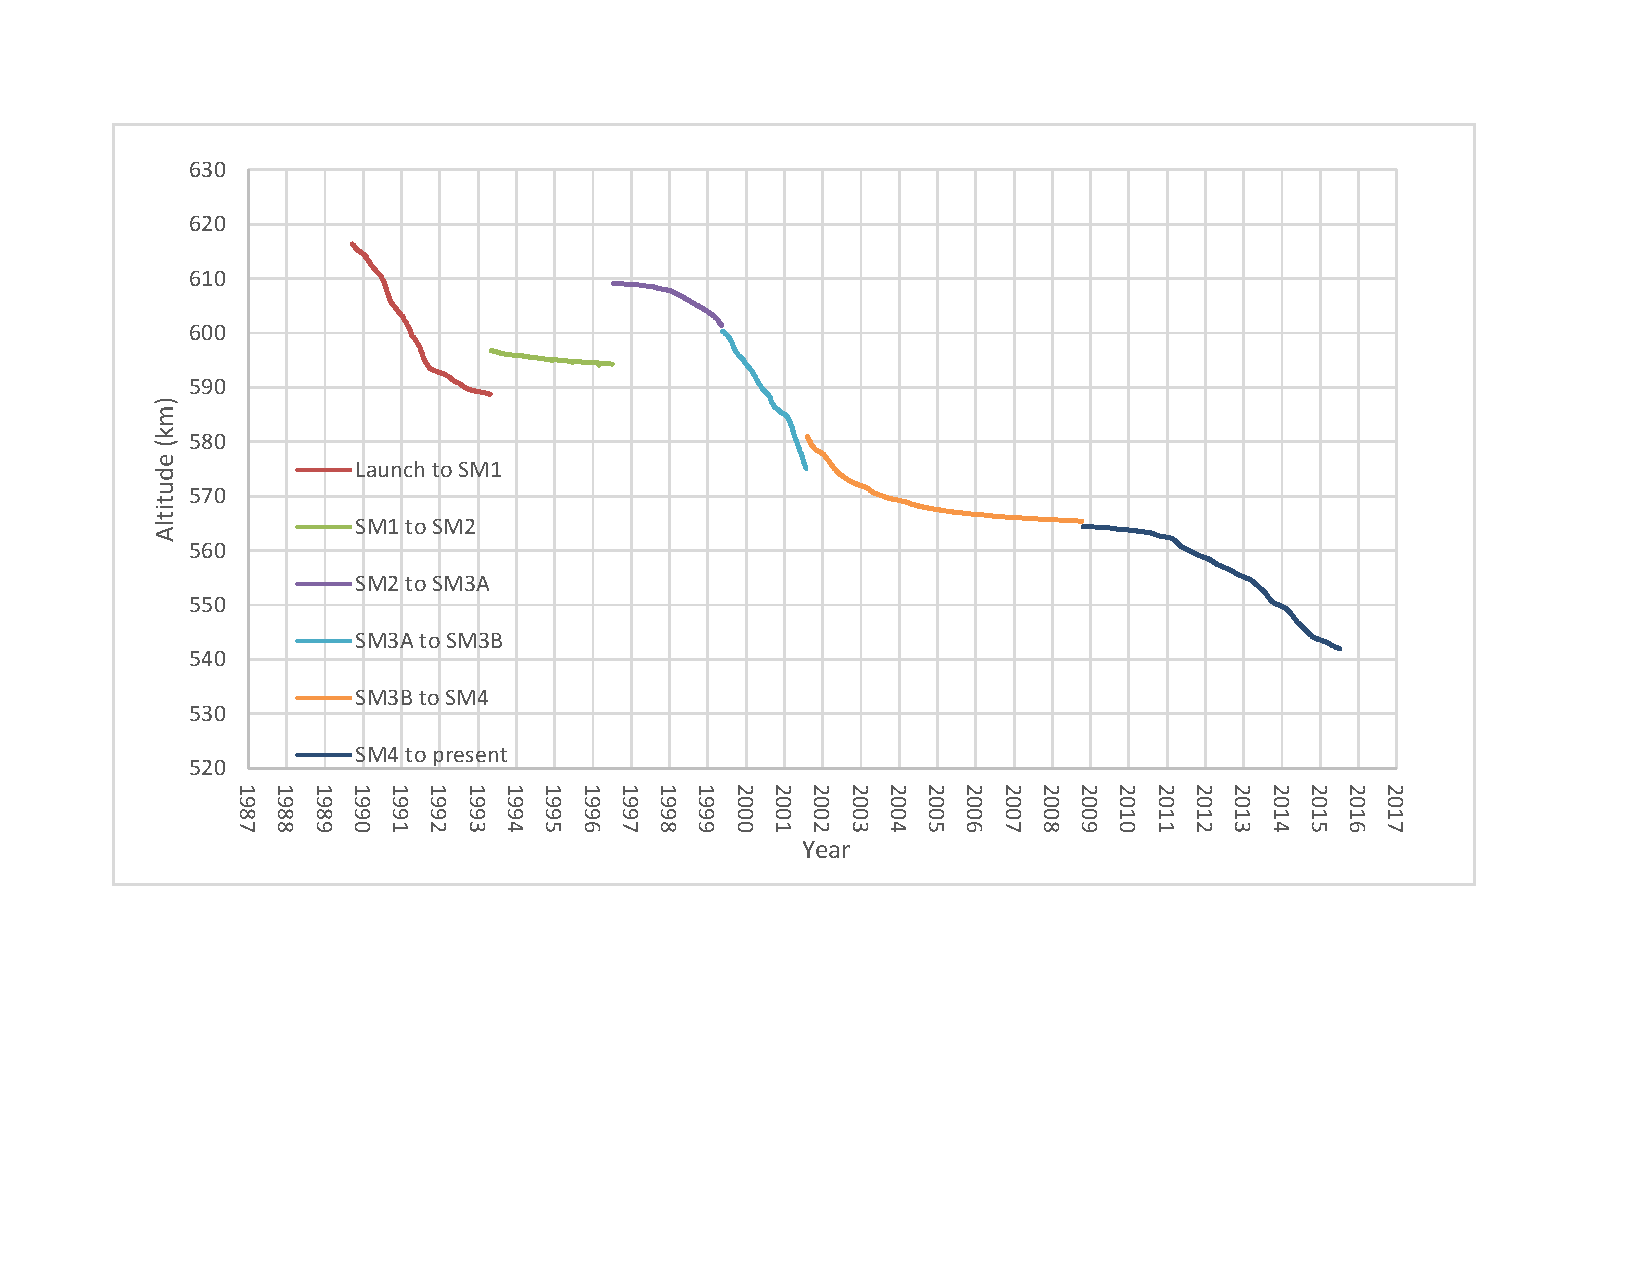
\includegraphics[width=1\textwidth]{recustomerrequirements/1.pdf}
\caption{Mean HST Altitude vs. Year}
\label{fig:fig1}
\end{center}
\end{figure}

As Figure~\ref{fig:fig1} shows\footnote{Note that the x-axis lines and labels displayed represent the midpoint of each year (approximately July 2 rather than January 1).}, the orbital decay of the satellite is not constant. The largest factor in the decay at this altitude is atmospheric drag, which itself is dependent on the solar cycle. During periods of increased solar activity, which can be approximated by the number of sunspots observed, the atmospheric density can be up to two orders of magnitude greater. This leads to a larger drag force on the satellite. As shown in Figure~\ref{fig:fig2} and Figure~\ref{fig:fig3}, the changes in number of sunspots correlates to the historical rate of change of orbital decay for the HST.

\begin{figure}[tb!]
\begin{center}
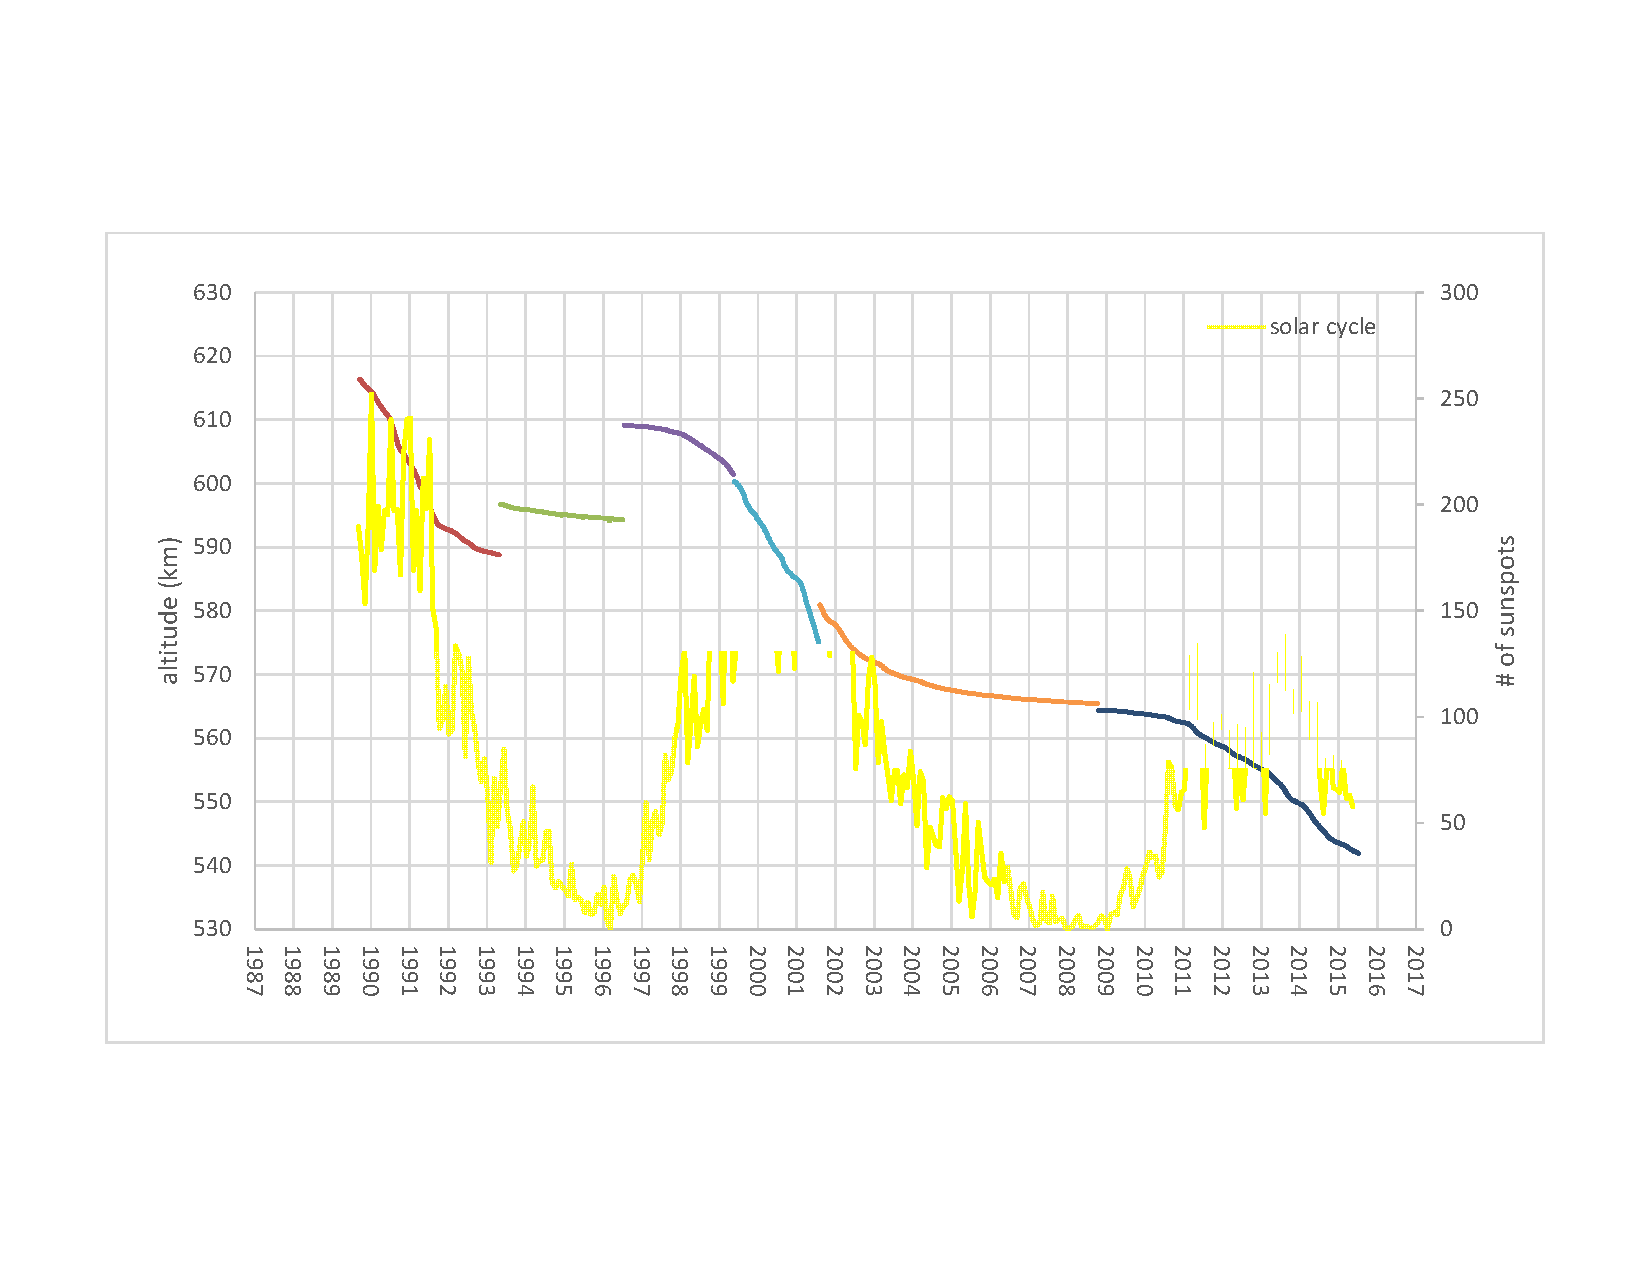
\includegraphics[width=1\textwidth]{recustomerrequirements/2.pdf}
\caption{Mean HST Altitude \& Solar Cycle vs. Year}
\label{fig:fig2}
\end{center}
\end{figure}

The rate of change of altitude can also be calculated using the TLE data, assuming that the orbit is approximately circular. Differentiating with respect to time (using the chain rule) gives the following:
\begin{align*}
\dfrac{d}{dt} h = \dfrac{d}{dt} a \dfrac{da}{dn} \dfrac{dn}{dt} = \dfrac{d}{dn} \mu^{\dfrac{1}{3}} n^{-\dfrac{2}{3}} \dfrac{dn}{dt} = -\dfrac{2}{3} \mu^{\dfrac{1}{3}} n^{-\dfrac{5}{3}} \dfrac{dn}{dt}
\end{align*}

where $\frac{dn}{dt}$ is also given by the TLEs. Therefore, rate of change of altitude ($\frac{dh}{dt}$) can also be plotted versus time and compared to the solar cycle data, as shown in Figure~\ref{fig:fig3}. Despite a large amount of transient error propagated through this calculation, there is a clear correlation between $\frac{dh}{dt}$ and the sunspot number.

\begin{figure}[tb!]
\begin{center}
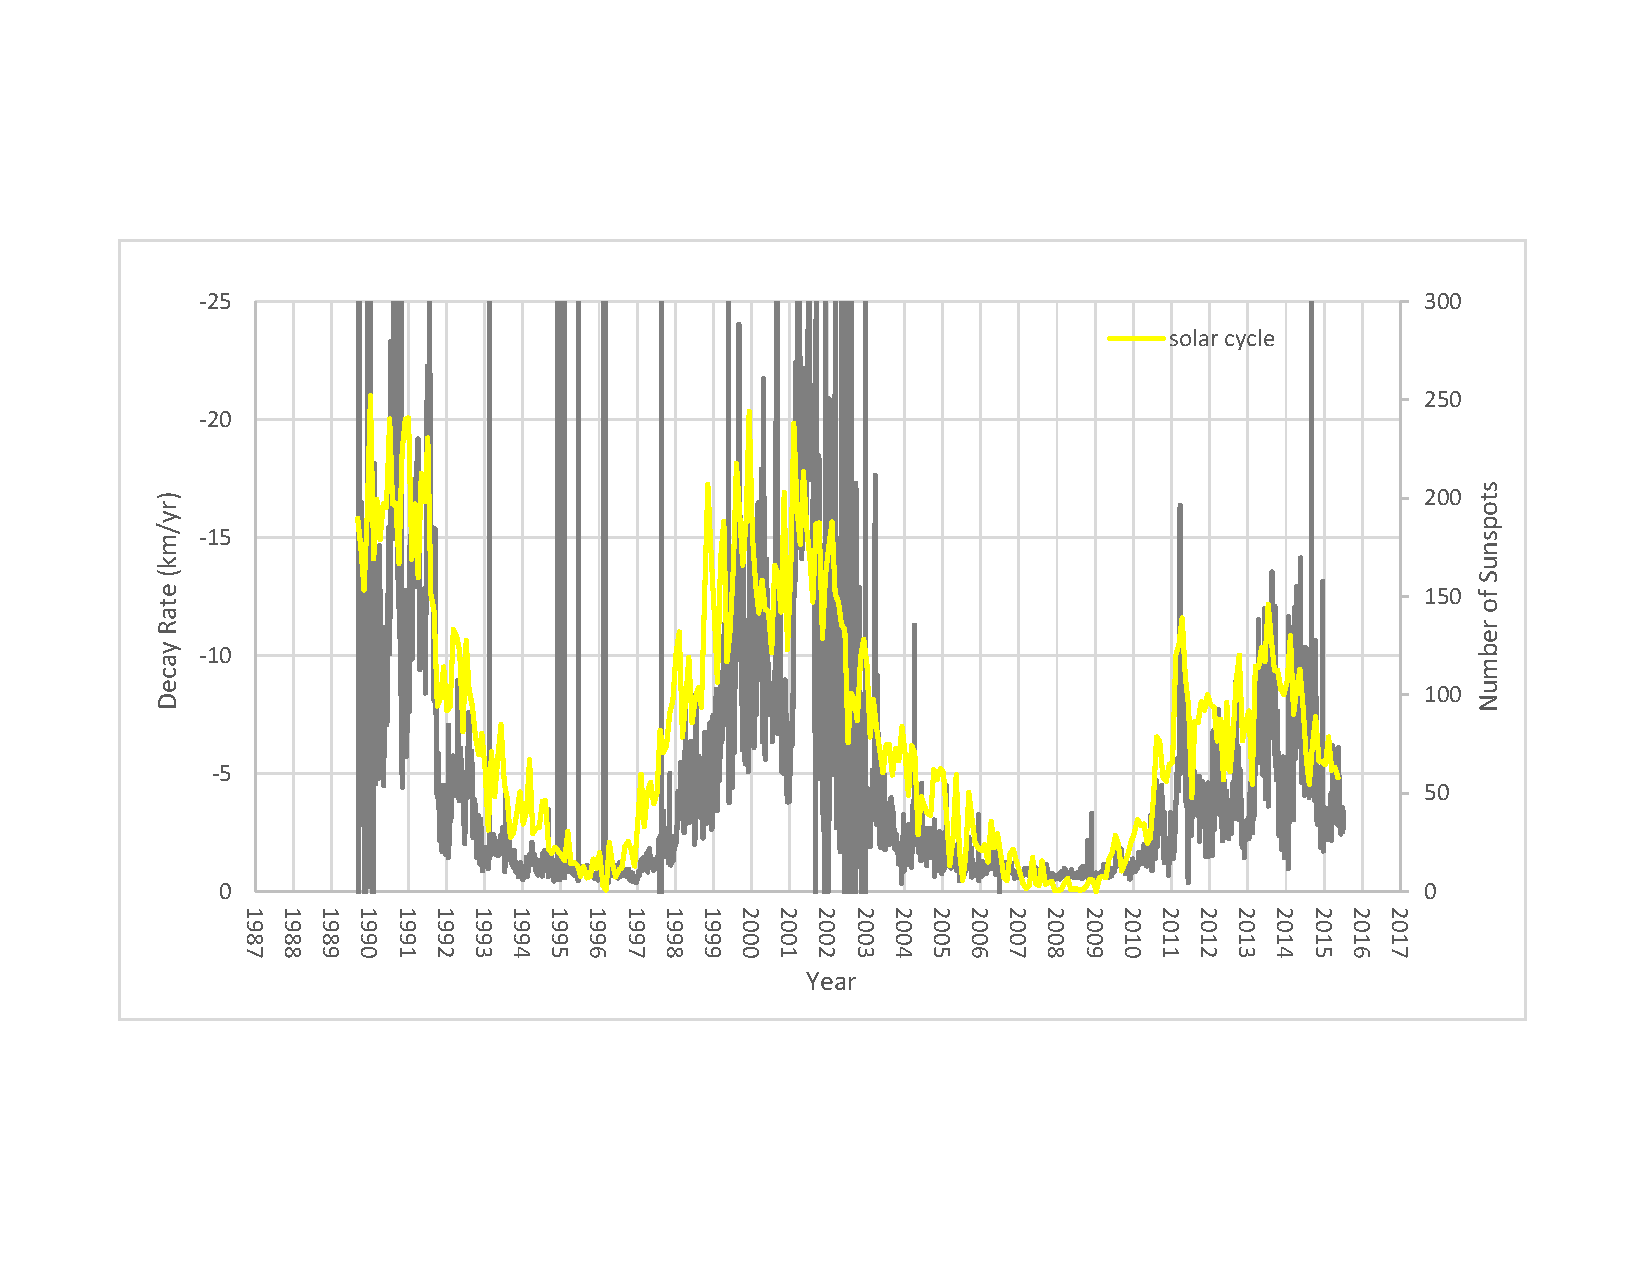
\includegraphics[width=1\textwidth]{recustomerrequirements/3.pdf}
\caption{Mean Altitude Decay \& Solar Cycle vs. Year}
\label{fig:fig3}
\end{center}
\end{figure}

\subsubsection{2020 Prediction}
The current solar cycle is significantly weaker than the previous two cycles, and appears to have already peaked. Therefore, it is expected that the HST orbital decay rate in the next few years will not be large. Figure~\ref{fig:fig3} shows that during periods of low solar activity, the decay rate can be as low as a kilometer per year. However, there is still a fair amount of uncertainty with regards to the future solar output and its effect on the satellite orbit, as hinted at by the amount of noise in the graph. Therefore, it would be wise to adopt a conservative approach during the preliminary design phase.

The HST altitude data was fitted in a few different ways in order to project to 2020. If the current decay rate were to continue with no decrease in solar cycle, the altitude would be 528 km --- however, this is an overly conservative estimate. If the decay rate matched that of the previous low periods, the altitude would be 536 km --- however, the previous periods were at a slightly higher altitude and this may not be steep enough, since decay rate decreases with altitude. Both of these scenarios are shown in Figure~\ref{fig:fig4}.

\begin{figure}[tb!]
\begin{center}
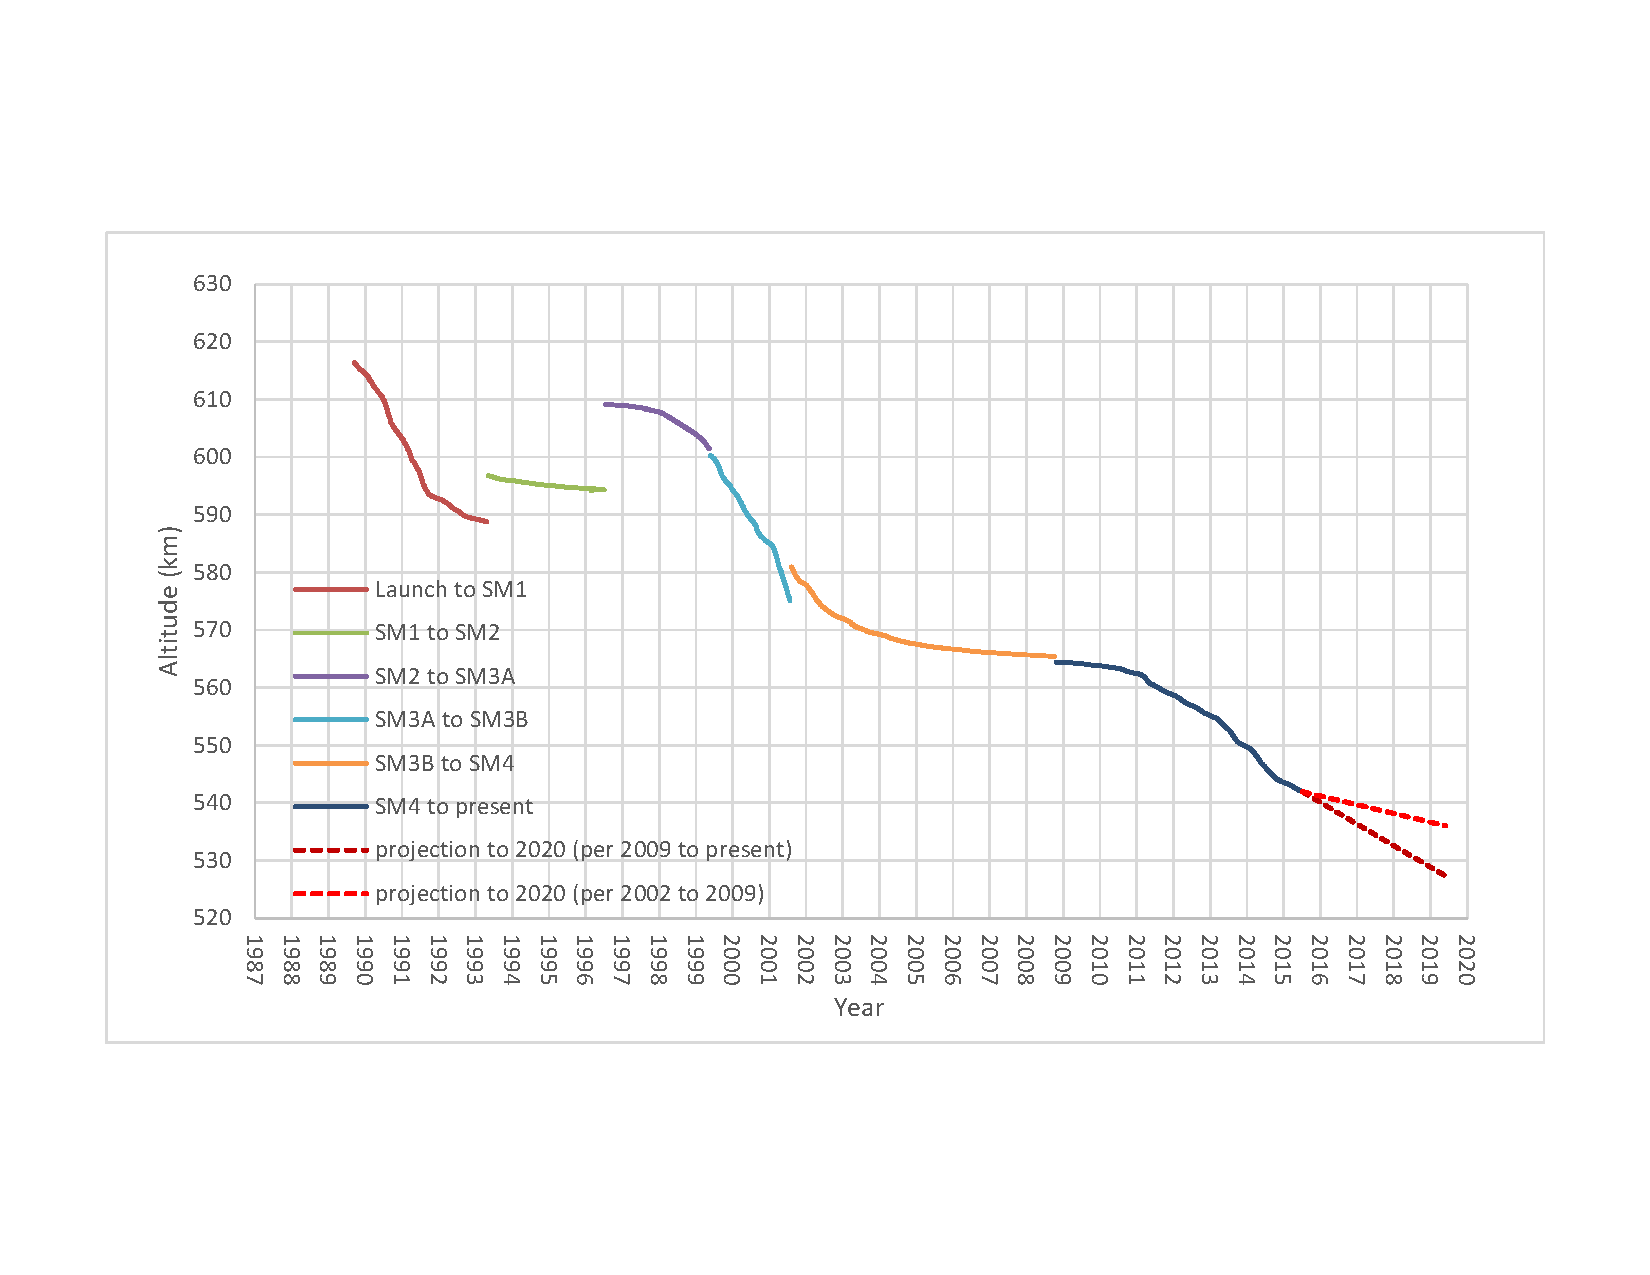
\includegraphics[width=1\textwidth]{recustomerrequirements/4.pdf}
\caption{Projected change in altitude}
\label{fig:fig4}
\end{center}
\end{figure}

An additional analysis was performed using AGI's Systems Took Kit (STK) software. STK was used to calculate the orbital elements for the HST from the present to 2028. The STK analysis does not account for a changing solar cycle model, but instead uses a drag estimate for the mean solar output. The STK model predicted a semi-major axis of 6910 km, corresponding to an altitude of 532 km in 2020, as shown in Figure~\ref{fig:fig5}.

\begin{figure}[tb!]
\begin{center}
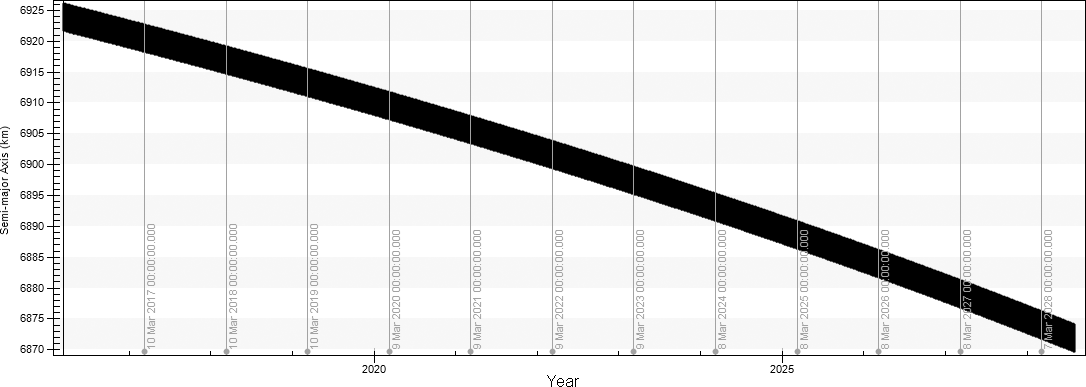
\includegraphics[width=1\textwidth]{recustomerrequirements/5.png}
\caption{STK altitude prediction}
\label{fig:fig5}
\end{center}
\end{figure}

The STK prediction falls neatly between the two previous predictions, therefore this altitude (532 km) was chosen for the mission.

\subsubsection{2028 Prediction}

The mission requirement is to re-boost the HST to a sufficient altitude so that it survives to October 2028. This involves predicting the decay rate at a number of possible re-boosted altitudes. However, future predictions become more difficult as the length of time is increased --- the solar cycle in particular is not easily predictable.

Figure~\ref{fig:fig5} also shows the HST altitude if no re-boost was done, which leads to the question of whether the re-boost is even necessary. Another solar maximum is expect to occur during this time frame, and the exact change in solar output is unknown. However, even without knowing the precise solar output over the next cycle, it appears likely that the HST could survive to 2028 on its own. This is partially due to the exceptionally weak current solar cycle.

Considering Hubble's history and considerable value even after the JWST is operational, it is desirable to continue HST's operation as long as possible. The HRV's sole purpose is re-boosting the HST and it must be designed large enough to interface with the HST regardless of the actual altitude. Because of these factors, it was decided to re-boost the HST as high as possible---back to its initial deployed altitude of 616 km. This will ensure the continuous operation of the HST to 2028 and well beyond.



\subsection{Communications}
\begin{enumerate}
\item The HRV shall have the ability to communicate with HST. (f)
\item The HRV shall have the ability to communicate with ground control through TDRS. (g)
\item The HRV shall have multiple rad tolerant processors. (h)
\item The HRV shall store sufficient power. (j)
\item The HRV shall generate sufficient power. (j)
\item The HRV shall have a failsafe to safely deorbit in case of communication loss. (m)
\item The HRV shall have the ability to stay within acceptable thermal ranges. (j)
\end{enumerate}

\section{Systems Requirements}
\subsubsection{Electronics/Power}
\begin{enumerate}
\item Minimum of three processors on C\&DH (h)
\item Failsafe program to deorbit the HRV in case of communication loss (m)
\item Solar Panels for energy generation (j)
\item Primary and backup battery cells for power storage (j)
\end{enumerate}
\subsubsection{Communications}
\begin{enumerate}
\item S-band antenna (f)
\item Ku-band antenna (g)
\end{enumerate}
\subsubsection{Thermal}
\begin{enumerate}
\item Thermal radiators to expel excess heat (j)
\end{enumerate}

\subsubsection{Rendezvous and Docking}
There is one customer requirement to consider in designing the rendezvous and docking. \say{(b), Rendezvous and dock with HST}.

To address this customer requirement, several system level requirements are set
\begin{enumerate}
\item A rendezvous plan shall be established.
\item A docking plan shall be established.
\item The rendezvous and docking plan shall have sufficient flight heritage.
\item Sufficient sensors shall exist to measure the state of the HRV for both absolute and relative navigation during rendezvous and docking.
\item Sufficient knowledge and control over the vehicle state shall be present in order to meet soft capture mechanism (SCM) docking requirements.
\end{enumerate}

\subsubsection{Propulsion}
The propulsion requirements for the mission depend on the maneuvering required for each phase. The propulsion requirements for each phase of the mission can be summarized as follows:

\begin{table}[h!]
\begin{center}
\begin{tabular}{l l r}
\toprule
Mission Phase & Propulsion Req'ts & $\Delta V$ (m/s) \\
\midrule
\makecell{1. Launch (delivered to parking \\ orbit)} & \makecell{The HRV shall carry enough \\ propellant to make up for orbital insertion inaccuracy (-30 km)}. & (included in phase 3) \\
\makecell{2. Maintain parking orbit for necessary phasing time} & \makecell{The HRV shall carry enough propellant to overcome perturbations \& dodge debris}. & \textbackslash150 \\
\makecell{3. Transfer to HST altitude} & \makecell{The HRV shall do a Hohmann transfer (two burns) to the HST altitude}. & 207 \\
\makecell{4. Rendezvous and dock with the HST} & \makecell{The HRV shall use cold gas thrusters to avoid damage or contamination to HST (refer to Rendezvouz and dock section)}. & \textbackslash50 \\
\makecell{5. Boost HST to new orbit} & \makecell{The HRV shall do a Hohmann transfer (two burns) w/ HST attached. The re-boost acceleration shall not damage the HST} & 46 \\
\makecell{6. Undock and separate from HST} & \makecell{The HSTRV shall use docking spring and cold gas thrusters to avoid damage or contamination to HST (refer to Rendezvouz and dock section).} negligible \\
\makecell{7. Maintain orbit for necessary phasing time & The HSTRV shall wait carry enough propellant to overcome perturbations while waiting for de-orbit window}. & negligible \\
\makecell{8. De-orbit to burn up in the atmosphere & The HSTRV shall do a 1/2 Hohmann transfer (1 burn) to de-orbit to the upper atm (120 km) over the ocean}. & 140 \\
\bottomrule
& Total $\Delta V$ & 596 \\
\bottomrule
\end{tabular}
\end{center}
% \caption{}
% \label{properties}
\end{table}



\chapter{Component Breakdown}
\section{Product Breakdown Structure}

\chapter{FMEA}
\chapter{Propulsion}

\chapter{Rendezvous and Docking}

\section{Docking}
\subsection{Small Autonomous Satellites}
There have been incredible advancements within the realm of semi-autonomous satellites over the past 20 years. Beginning in 1997, the Autonomous Extravehicular Activity Robotic Camera Sprint (AERCam Sprint) was the first semi-autonomous satellite to demonstrate the use of a free-flying prototype camera aboard the International Space Station (ISS). While operating alongside STS-87 Mission Specialist Winston Scott, the AERCam Sprint flew under the remote-control guidance of Steve Lindsey for approximately 75 minutes, and relayed live television images to Columbia's Mission Control~\cite{Aercam,MiniAercam}. After successfully completing this experiment, researchers and analysts decided to incorporate a higher level of autonomy, and produced a second prototype known as the Mini AERCam in 2000. While this satellite never made it to space, the Mini AERCam underwent multiple tests on an air-bearing table and in an orbital test simulation facility at Johnson Space Center. This newly designed satellite was given automatic position hold, point-to-point maneuvering, and an additional camera to provide an orthogonal view, allowing astronauts to navigate the Mini AERCam with respect to the ISS. Through these multiple additions, researchers expanded the satellite's capability to encompass supervised autonomous and/or remotely piloted operations~\cite{MiniAercam,MiniAercam2}.

In 2006, the first Synchronized Position Hold Engage Reorient Experiment Satellites (SPHERES), a self-contained nanosatellite made by MIT's Space Systems Laboratory, was launched to the ISS and taken to the US Laboratory. Since that time, this semi-autonomous satellite has been joined by two additional SPHERES, making this system the first consistent experimental nanosatellite testbed aboard the ISS. Unlike the AERCam Sprint and the Mini AERCam, SPHERES is a modular satellite where each system is self-contained in individual capsules. This configuration allows SPHERES to easily incorporate system expansions onto specific platforms, such as navigation, without needing to reconfigure the entire craft. Furthermore, its modularity helps researchers efficiently address system failures, making it easier for astronauts to perform on-site repairs. To navigate SPHERES within the ISS, the system utilizes wall-mounted ultrasonic beacons and corresponding ultrasonic receivers attached to the nanosatellite~\cite{SPHERES}. SPHERES emits an infrared flash to determine its location. Once emitted, the satellite waits for the wall-mounted beacons to emit corresponding ultrasonic pulses. After receiving these ultrasonic pulses, the satellite measures its range based on the pulse's time of flight, and can then calculate its relative position, attitude, and angular velocity~\cite{SPHERES,Vertigo1}. This unique navigation system allows SPHERES to emulate a ``pseudo-GPS'' time-of-flight sensing system, and ultimately estimate its position, angular velocity, and attitude without the potential for signal interference and noise -- a challenge that has been previously encountered with GPS systems~\cite{Vertigo1}. Through this autonomous navigation and modular design, the SPHERES testbed has become a versatile platform for developing vision-based navigation, anti-collision, and formation flying algorithms. By allowing research teams to create algorithms that can then be uplinked to the SPHERES test system aboard the ISS, researchers can receive live feedback, and ultimately find the exact areas within their algorithms that need improvement.

\subsubsection{SPHERES VERTIGO}
In 2008 the MIT Space Systems Laboratory began building an upgrade to the SPHERES system, known as the Low Impact Inspection Vehicle (LIIVe), as part of the Visual Estimation and Relative Tracking for Inspection of Generic Objects (VERTIGO) program. Once completed, this upgrade would later be attached to the existing SPHERES system and act as VERTIGO ``goggles,'' allowing SPHERES to perform vision-based navigation experiments in the microgravity environment aboard the ISS. After adjusting these VERTIGO Goggles to suit the space station's environment, the final system was upgraded to include two monochrome stereo cameras, two illuminating LEDs, a 1.2 GHz Via Nano processor, an 802.11n network card, and optics that included a larger aperture lens in a synchronized stereo configuration~~\cite{SPHERES,Vertigo1,Vertigo2,Vertigo3}.

When the modified SPHERES VERTIGO was ready for experimentation, numerous flight algorithms were tested to demonstrate the spacecraft's complete autonomy. After ISS Expedition 34, it was confirmed that SPHERES VERTIGO was capable of autonomously conducting a circular orbit about an uncooperative object, while simultaneously maintaining a constant relative position between SPHERES VERTIGO and the target. This objective was achieved through the primary use of inertial sensors and cameras, and was considered an unprecedented success~\cite{Vertigo2,Vertigo3}.

\subsection{Collision Avoidance and Docking Algorithms}
Since the SPHERES nanosatellite's first microgravity guidance, navigation, and control experiment, there have been three classes of algorithms pertaining to collision avoidance and docking that have emerged: metrology, control, and autonomy~\cite{SPHERES_form}.

The metrology algorithms were implemented using a SPHERES-specific interface, and utilized a series of Extended Kalman Filters to obtain the system's state vector from the sensor outputs. This approach has been typically utilized in position, attitude, and determination systems. Despite many successful implementations, recent literature suggests that the second and third classes have demonstrated greater accuracy in the areas pertaining to collision avoidance and docking~\cite{SPHERES_form}.

The control algorithm class involves both closed-loop controls and path-planning algorithms. One prominent control algorithm that has been frequently tested is the glideslope algorithm. This algorithm is a hybrid between a path-planning and a velocity-control algorithm, where the incoming spacecraft is given commands to slow its velocity as it approaches its target~\cite{SPHERES_form,SPHERES_micro,dist,virt_sim}. The glideslope algorithm was the first autonomous docking algorithm to successfully attach an incoming spacecraft to its tumbling target, and is a relatively simple, yet robust, controller makes this algorithm~\cite{SPHERES_micro}. Another promising algorithm is the ``safe'' trajectory algorithm. This innovative algorithm computes a pre-planned trajectory using the solution from a Mixed-Integer Linear Program, and, using this pre-computed trajectory, is able to optimize fuel and avoid incoming obstacles~\cite{SPHERES_micro}. However, while this algorithm is guaranteed to produce a safe trajectory, its overall complexity requires it to be computed on an external computer. Once the computations have been completed, the final trajectory is transferred to the satellite. This entire computational process creates an approximate nine second delay, and can potentially create a catastrophic outcome if the spacecraft requires an immediate trajectory path to avoid an incoming collision. To remedy this solution, researchers have begun to trade trajectory and fuel optimality for computational time, and can reduce the total computation time to about $0.17$ seconds~\cite{SPHERES_micro}. Lastly, the ``close point of approach'' algorithm has been demonstrated to be both compact and computationally efficient, and has served as a background safety routine for the high school SPHERES Zero Robotics program~\cite{virt_sim}. While all three aforementioned algorithms have accurately performed numerous tests pertaining to collision avoidance and docking, each algorithm is associated with its own specific set of pros and cons. As it currently stands, researchers have yet to find a way to optimize fuel usage, pre-planned trajectories, and computational power, and thus must decide which factors are most important for any given mission~\cite{SPHERES_form,SPHERES_micro,dist,virt_sim}.

Finally, the autonomous algorithm class is used to execute the control class algorithms and determine the current mode of operation~\cite{SPHERES_form}. As a result, the glideslope, ``safe'' trajectory, and ``close point of approach'' algorithms all utilize autonomy to properly perform their respective procedures.

\subsection{Autonomous versus manual docking}
In recent years the small satellite platform has increased in popularity. With the ability to launch multiple small satellites as a secondary payload and the relatively low development cost involved, they are one of the most viable testbeds for new technologies. One great example of this is the class of satellites that adhere to the CubeSat standard~\cite{CubeSat}. CubeSat initiatives have made many projects possible due to the minimal costs required. Although a small size limits their capabilities, higher fidelity projects usually require a larger volume to contain all desired systems. There are several projects that use slightly larger free flyers that have produced unique navigation demonstrations such as AERCam Sprint, Mini-AERCam, and SPHERES ~\cite{Aercam,MiniAercam,SPHERES}. While the Hubble Reboost Vehicle (HRV) is significantly larger than the aforementioned satellites, the rendezvous and docking algorithms developed for these missions can be made just as effective.

These projects make use of an optical sensor to take stereoscopic visual recordings for inspection purposes, and to determine the position and attitude in relation to a target. To do this, the image captured must be used in conjunction with a computer vision algorithm in order to estimate navigational parameters. Using a two color cameras and the full visual light spectrum, a more familiar virtual image is produced. Operators are able to view the subject as if it was in front of them, allowing for quick and informed decision making. This, as among other reasons, has been realized by many research teams and can be seen in many projects such as SPHERES VERTIGO and the aforementioned AERCam projects~\cite{Aercam,MiniAercam,Vertigo1}.

Most current docking procedures utilize a laser range finder for determining distance. Laser range finders have flight heritage and have moderate accuracy~\cite{Docking}. Simple fiducial markers can be used to increase the performance of range finders, and multiple markers can allow rangefinders to triangulate a relative position. Markers for visual navigation systems, however, can vary in complexity. Marker distribution and marker shape can allow a computer vision system to gather a large amount of data with a single image, whereas a laser rangefinder must take multiple measurements. This system was originally developed for manual docking operations, but it also provides visual information to allow more accurate computer vision position measurements.

In ground-based scenarios, the only drift from the intended rendezvous trajectory is contributed to error or disturbances, but in this situation there is also drift due to the inspector and the target occupying different orbits. Even with a perfect initial trajectory and planning, corrections are required. The navigation scheme must be as efficient as possible as course corrections are unavoidable.

The great distances involved in satellite operation, coupled with an inherent delay involved with routing signals to a ground station, however, make human operation of the HRV infeasible. A one-way time delay of a few seconds from a satellite to the ground-based operator, with the addition of just one second of human operator delay, with the additional delay of a few seconds back from the ground-based operator to the satellite result of time delays greater than 5-10 seconds, at which point it is too late to make corrections. An automated system, based on the navigation schemes outlined above, has a much greater chance for success. Such a system can make nearly instantaneous decisions, and can execute them before a human operator has time to identify the situation. Coupling an automated docking procedure with a human backup to abort gives the best of both scenarios. The automated docking system can handle the lower level task of docking, and the human operator is present to abort the docking attempt if unexpected errors occur.

\section{Rendezvous}

\subsection{How will we rendezvous, and how long does rendezvous take?}
\begin{figure}[t!]
\begin{center}
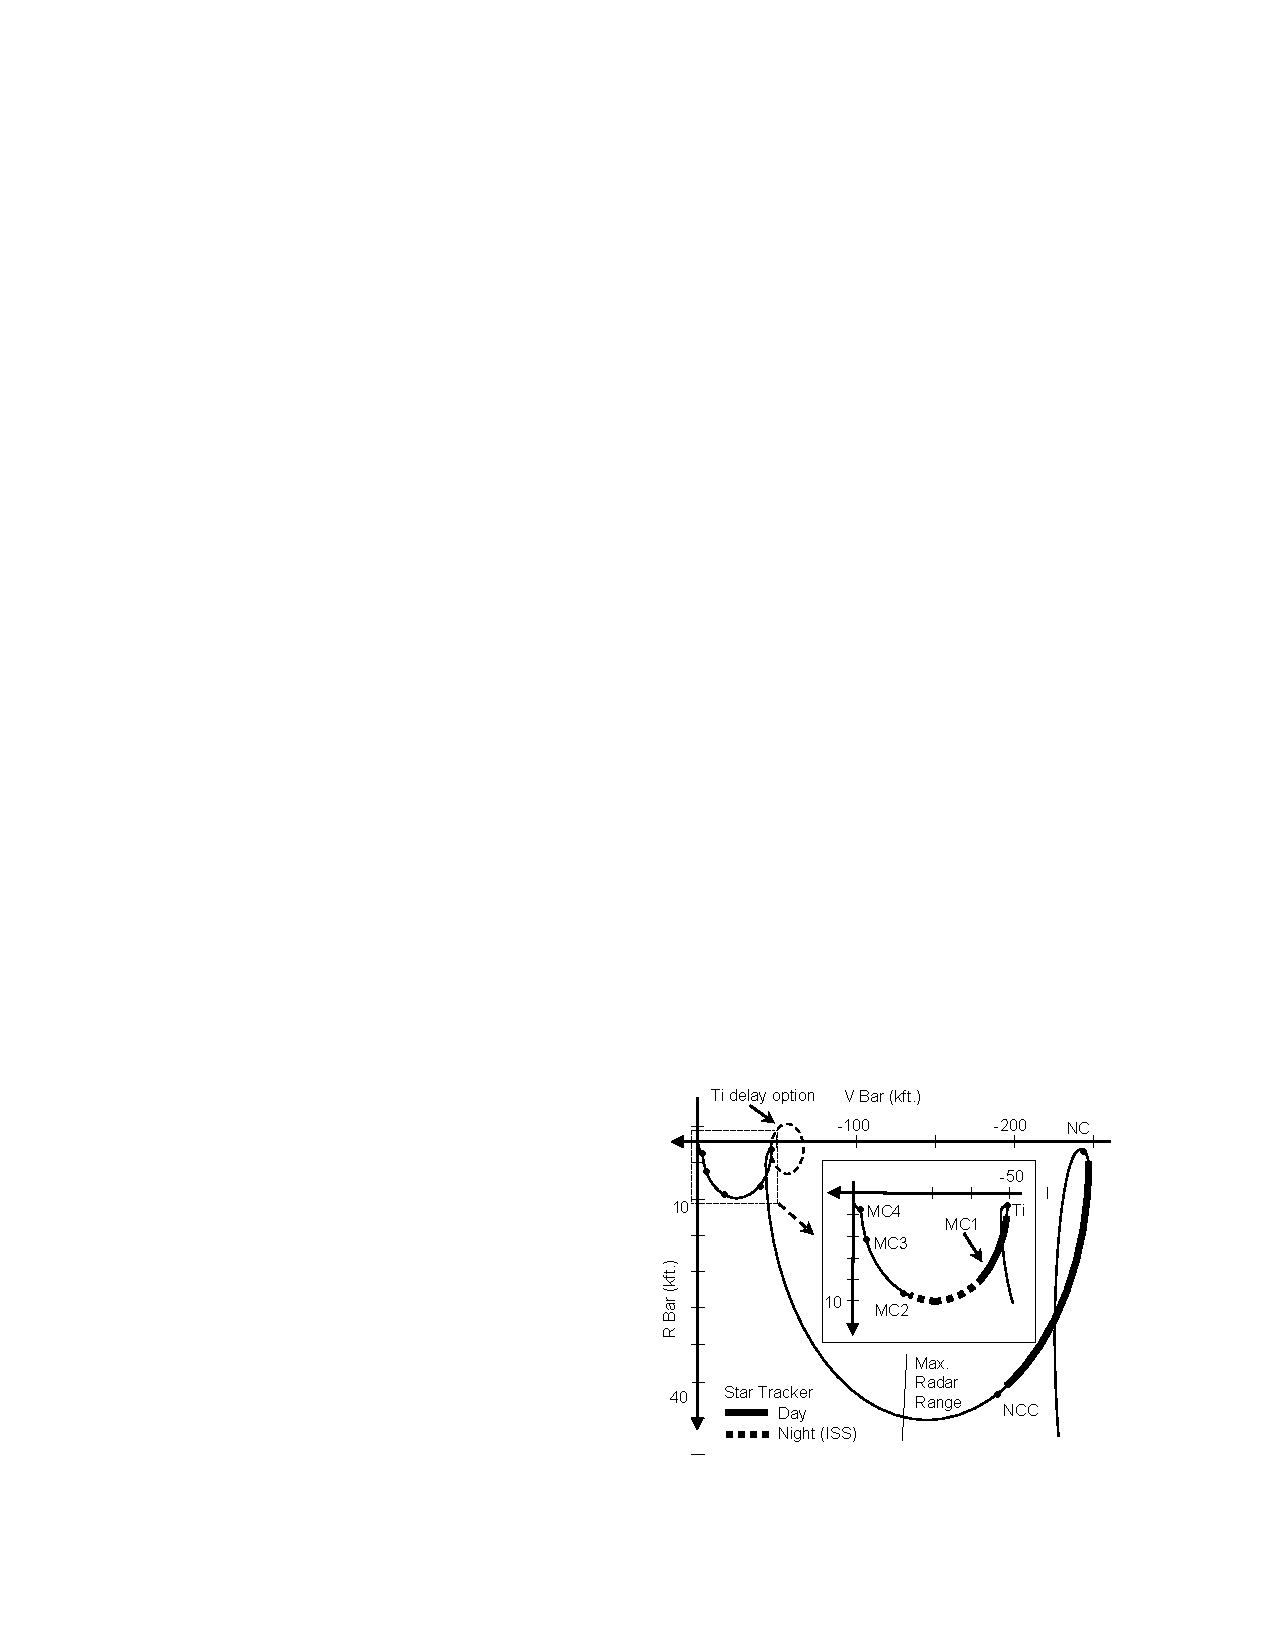
\includegraphics[width=.5\textwidth]{imgs/orbt.pdf}
\caption{Optimized R-Bar Targeted Rendezvous (ORBT) relative navigation rendezvous diagram.}
% \label{fig:density}
\end{center}
\end{figure}

Current orbital decay predictions place the Hubble Space Telescope (HST) at a nearly circular, 528 km altitude orbit during our proposed launch date of January 2020. After launch, we will enter a 200 km, in-plane parking orbit, then enter a 500 km phasing orbit. From our phasing orbit, we will perform a homing maneuver bring us to a holding point 15 km behind HST. When relative navigation sensors have acquired HST, we will perform a closing maneuver to bring us to 500 m below HST, after which an R-bar approach will be used to bring us to dock.

For the R-bar approach, our vehicle move up towards HST along its radial vector. Our vehicle will fire thrusters radially to close towards HST, and use small burns in the orbital velocity direction to negate the effects of orbital mechanics. If the R-bar is stopped at any point (in case of loss of communication or thruster failure, for instance), our vehicle will naturally move away from HST. If, at any point in the docking, communication is lost, the HRV will automatically return to a holding point behind HST.

This approach has been adapted from the from the Space Shuttle's Optimized R-Bar Targeted Rendezvous (ORBT) profile~\footnote{Goodman, John L. ``History of Space Shuttle Rendezvous.'' (2011).}. ORBT was developed to optimally set up initial conditions for a low energy coast up the +R-bar. This profile was used from 1997 to the end of Space Shuttle program in 2011, lending more than a decade of operational flight heritage.

\subsection{At what stage of the rendezvous are sensors active? Can we recover from a single sensor failure at each stage?}
\begin{table}[tb]
\begin{center}
\begin{tabular}{c c c c}
\toprule
Sensor & \# On-board & Upper Range & Lower Range \\
\midrule
Radar        & 2 & 100s of km & 100s of m  \\
LIDAR        & 2 & 10s of km & 2m  \\
Camera       & 2 & 100s of m & contact  \\
GPS          & 2 & - & -  \\
\bottomrule
\end{tabular}
\end{center}
\caption{Relative and absolute navigation sensors onboard the HRV.}
% \label{properties}
\end{table}

\begin{table}[tb]
\begin{center}
\begin{tabular}{c c c c}
\toprule
Sensor & \# On-board & Performance \\
\midrule
Horizon Sensor & 2 & 0.25 deg \\
Sun Sensor     & 1 & 0.01 deg \\
Startracker    & 2 & 0.005 deg \\
IMU            & 2 & 0.003 deg/hr \\
\bottomrule
\end{tabular}
\end{center}
\caption{Attitude measurement sensors onboard the HRV.}
% \label{properties}
\end{table}

The most likely cause of failure for our spacecraft is a loss of attitude measurement. When the spacecraft is phasing with HST, its sources of attitude measurement are startrackers, a sun sensor, horizon sensors, and IMUs. Without frequent updates from the other attitude sensors, however, the IMUs experience drift and quickly become useless. Once the spacecraft comes within a few 10s of km of HST, however, radar and LIDAR can also be used calculate relative attitude. During final approach, the last few 100 m, stereo cameras can calculate sufficient pose estimation for docking.

There are at least two sensors available at all times for both attitude and navigation during all parts of the mission. During all phases of the mission, except for final rendezvous and docking, GPS navigation is sufficient to navigate. Once we begin the final stages of rendezvous and docking, there are three types of relative navigation sensors available. Two redundant radar sensors can be used to initially make relative navigations, and we can transition to LIDAR and optical measurements for the final 100s of meters. Horizon and sun sensors, and star trackers can be used for absolute attitude measurement for the early stages of the mission, and LIDAR and optical measurements can be used for relative pose navigation during the final stages of docking.

\begin{table}[tb]
\begin{center}
\begin{tabular}{c c c c}
\toprule
Sensor & Displacement Error & Rate Error \\
\midrule
Lateral   & 11.4 cm & 1.3 cm/s \\
Range     & 20.3 cm & 5.1 cm/s \\
Roll      & 4 deg   & 1 deg/s \\
Pitch/Yaw & 4 deg   & 0.25 deg/s \\
\bottomrule
\end{tabular}
\end{center}
\caption{}
% \label{properties}
\end{table}


\subsection{How long can we stay at each part of the orbit?}

If sufficient time has passed without contact with ground control, the HRV should automatically perform a deorbit burn. If additional failures, such a major electrical issue, prevent the HRV from deorbiting, there is a possibility of remaining in orbit for much longer than the intended mission duration.

Various orbital perturbations such as gravity gradients, solar pressure, magnetic field interactions, and atmospheric drag can decrease the altitude of the orbit. Of these factors, the largest for low Earth orbit is drag, which increases exponentially as the spacecraft lowers altitude. The acceleration due to drag is
\begin{align*}
D &= \dfrac{1}{2} \rho v^2 A C_d
\end{align*}
in the direction opposite of the spacecraft's velocity. Here $\rho$ is the density of the atmosphere, $A$ is the area exposed to the atmosphere, and $C_D \approx 2.2$ is the coefficient of drag. The solar radio flux can also change dramatically with the solar cycles, and has strong affects on the atmosphere. A program was developed under the assumptions of constant satellite mass, LVLH attitude, and $C_D$. $\rho$ is modeled as an exponential factor based on altitude.

There are three main circular orbits that the mission will take place in: 200km orbit, 536km orbit, and a 616km orbit. As the satellite boosts itself (and Hubble) to higher, it expends fuel, which means that our satellite will always have a lower mass at higher orbits. The results and input parameters of the orbit lifetime analysis are listed in Table~\ref{altitude_table}. Satellites will remain in orbit longer at higher altitudes, where the atmospheric density is lowest. As such, the longest orbital lifetimes are at highest orbit, and the shortest lifetimes are at low altitudes. If satellite communication is not established within the first three days, the HRV will destructively re-enter the atmosphere.

% \begin{table}[tb]
% \begin{center}
% \begin{tabular}{rrrrr}
% \toprule
% Altitude & 200km & 536km & 616km \\
% \midrule
% $m$ & 996 kg & 881 kg & 637 kg \\
% $t$ & 2.9 days & 99.5 years & 380 years \\
% \bottomrule
% \end{tabular}
% \end{center}
% \caption{$C_D$=2.2, $A=4$m$^2$}
% \label{altitude_table}
% \end{table}

\begin{table}[tb]
\begin{center}
\begin{tabular}{lrrrrr}
\toprule
Mass (kg) &           600  &           700  &           800  &           900  &           1000 \\
Altitude (km)     &                &                &                &                &                \\
\midrule
100.0 &       0.3 &       0.3 &       0.4 &       0.4 &       0.4 \\
237.5 &      12.4 &      14.4 &      16.5 &      18.5 &      20.5 \\
375.0 &     544.7 &     635.4 &     726.1 &     816.8 &     907.5 \\
512.5 &   15073.3 &   17585.4 &   20097.5 &   22609.6 &   25121.7 \\
650.0 &  257994.8 &  300993.8 &  343992.8 &  386991.8 &  429990.8 \\
\bottomrule
\end{tabular}
\end{center}
\caption{Time to deorbit, in days with $C_D$=2.2, $A=4$m$^2$.}
\label{altitude_table}
\end{table}

\lstinputlisting[caption=Orbital decay python script.]{decay.py}

\chapter{Historical Data}

% \begin{table}[h]
% \begin{center}
% \begin{tabular}{|c |c |c |c |c|}
% % \toprule
% \hline
% Maneuver & Time, MET & System & $\Delta$V, ft/sec & Duration, sec \\
% % \midrule
% \hline
% NC-1  & 00:05:27:28.9 & OMS (Both) & 98.0 & 59.2 \\ \hline
% NSR   & 01:03:43:59.7 & OMS (Both) & 49.8  & 30 \\ \hline
% NC-2  & 01:04:17:14.3 & OMS (Left) & 14.1 & 17.1 \\ \hline
% NC-3  & 01:17:55:30.1 & OMS (Right) & 12.1 & 14.8 \\ \hline
% % \bottomrule
% \end{tabular}
% \end{center}
% \caption{STS-61. The HST was grappled at 01:23:19:56 and berthed at 01:23:57:30.}
% % \label{properties}
% \end{table}

% % \begin{table}[h]
% % \begin{center}
% % \begin{tabular}{|c |c |c |c |c|}
% % % \toprule
% % \hline
% % Maneuver & Time, MET & System & $\Delta$V, ft/sec & Duration, sec \\
% % % \midrule
% % \hline
% % Reboost 1  & 06:16:59 & RCS Vernier (?) & - & 61 \\ \hline
% % % \bottomrule
% % \end{tabular}
% % \end{center}
% % \caption{STS-61. The HST was grappled at 01:23:28 and berthed at 2:00:10.}
% % % \label{properties}
% % \end{table}

% \begin{table}[h]
% \begin{center}
% \begin{tabular}{|c |c |c |c |c|}
% % \toprule
% \hline
% Maneuver & Time, MET & System & $\Delta$V, ft/sec & Duration, sec \\
% % \midrule
% \hline
% NSR   & 01:03:36:21.9  & OMS         & 96  & 56.2 \\ \hline
% NC-2  & 01:05:02:00    & RCS Primary & 3.1 & 13.0 \\ \hline
% NH    & 01:17:06:04.9  & OMS         & 12  & 8.0  \\ \hline
% NC-3  & 01:17:53:00    & RCS Primary & 3.4 & 14.0 \\ \hline
% NPC-2 & 01:19:00:24    & RCS Primary & 0.5 & 2.0  \\ \hline
% NCC   & 01:20:07:46    & RCS Primary & 1.1 & 1.1  \\ \hline
% TI    & 01:21:07:52    & RCS Primary & 2.8 & 12.0 \\ \hline
% MC-1  & 01:21:34:16    & RCS Primary & 0.4 & 2.0  \\ \hline
% MC-2  & 01:22:02:40    & RCS Primary & 1.5 & 6.0  \\ \hline
% MC-3  & 01:22:12:40    & RCS Primary & 0.9 & 3.0  \\ \hline
% MC-4  & 01:22:22:40    & RCS Vernier & 0.2 & 1.0  \\ \hline
% % \bottomrule
% \end{tabular}
% \end{center}
% \caption{STS-82. The HST was grappled at 01:23:28 and berthed at 2:00:10.}
% % \label{properties}
% \end{table}

% % \begin{table}[h]
% % \begin{center}
% % \begin{tabular}{|c |c |c |c |c|}
% % % \toprule
% % \hline
% % Maneuver & Time, MET & System & $\Delta$V, ft/sec & Duration, min:sec \\
% % % \midrule
% % \hline
% % Reboost 1 & 04:01:09:28 & RCS Vernier & 6.6  & 20:41.9 \\ \hline
% % Reboost 1A$_a$ & 04:06:07:04 & RCS Vernier & 3.3  & 10:12.6 \\ \hline
% % Reboost 2 & 5:01:15:03 & RCS Vernier & 6.5  & 19:46.9 \\ \hline
% % Reboost 3 & 07:01:33:00 & RCS Vernier & 10.4 & 31:53.5 \\ \hline
% % % \bottomrule
% % \end{tabular}
% % \end{center}
% % \caption{STS-82. a - Manuever required for space debris avoidance. The four reboost maneuvers raised the HST orbit an average of 8 nmi.}
% % % \label{properties}
% % \end{table}

\begin{table}[h]
\begin{center}
\begin{tabular}{|c |c |c |c |c|}
% \toprule
\hline
Maneuver & Time, MET & System & $\Delta$V, ft/sec & Duration, sec \\
% \midrule
\hline
NC-1 Trim & 01:03:42:23    & RCS Primary & 0.06 & 0.44   \\ \hline
NC-2      & 01:04:36:49    & RCS Primary & 7.4  & 31     \\ \hline
NSR Trim  & 01:17:36:55.1  & RCS Primary & 0.2  & 0.24   \\ \hline
NCC       & 01:20:38:00    & RCS Primary & 0.3  & 1.0    \\ \hline
TI        & 01:21:36:06    & RCS Primary & 4.1  & 8.7    \\ \hline
MC-1      & 01:21:58:06    & RCS Primary & 0.3  & 0.5    \\ \hline
MC-2      & 01:22:32:58    & RCS Primary & 0.9  & 2.9    \\ \hline
MC-3      & 01:22:49:58    & RCS Primary & 0.4  & 1.0    \\ \hline
MC-4      & 01:22:59:58    & RCS Vernier & 1.8  & 7.2    \\ \hline
% \bottomrule
\end{tabular}
\end{center}
\caption{STS-103. The HST was grappled at 01:23:44:01 and berthed at 2:00:52.}
% \label{properties}
\end{table}


\begin{table}[h]
\begin{center}
\begin{tabular}{|c |c |c |c |c|}
% \toprule
\hline
Maneuver & Time, MET & System & $\Delta$V, ft/sec & Duration, sec \\
% \midrule
\hline
NC2  & 000:17:50:50.5 & -X RCS & 4.5 & 19.7 \\ \hline
NC3  & 01:02:55:32    & Multi-axis RCS & 3.1 & 12.6 \\ \hline
NC4  & 01:17:47:01    & Multi-axis RCS & 4.8 & 20.4 \\ \hline
NCC  & 01:18:38:57    & Multi-axis RCS & 1.3 & 5.5 \\ \hline
MC-1 & 01:19:59:04    & Multi-axis RCS & 0.8 & 3.2 \\ \hline
MC-2 & 01:20:34:27    & Multi-axis RCS & 0.4 & 1.79 \\ \hline
MC-3 & 01:20:34:27    & +X RCS & 1.9 & 8.1 \\ \hline
MC-4 & 01:21:01:28    & Multi-axis RCS & 1.9 & 8.1 \\ \hline
% \bottomrule
\end{tabular}
\end{center}
\caption{STS-109. The HST was captured at 001:21:09:19.}
% \label{properties}
\end{table}

% \begin{table}[h]
% \begin{center}
% \begin{tabular}{|c |c |c |c |c|}
% % \toprule
% \hline
% Maneuver & Time, MET & System & $\Delta$V, ft/sec & Duration, min:sec \\
% % \midrule
% \hline
% Reboost 1 & 07:05:56:01.8 & RCS Vernier (?) & 11.8  & 36:00 \\ \hline
% % \bottomrule
% \end{tabular}
% \end{center}
% \caption{STS-109. The reboost maneuver raised the HST orbit an average of 3.6 nmi.}
% % \label{properties}
% \end{table}

\begin{table}[h]
\begin{center}
\begin{tabular}{|c |c |c |c |c|}
% \toprule
\hline
Maneuver & Time, GMT & System & $\Delta$V, ft/sec & Duration, sec \\
% \midrule
\hline
NC 1 & 131/21:49:54.65 & RCS & 19.5 & 90.88   \\ \hline
NCC  & 133/13:41:50    & RCS &  1.6 & 7.0     \\ \hline
MC 3 & 133/15:53:26.3  & RCS &  0.9 & 0.2     \\ \hline
MC 4 & 133/16:03:26.5  & RCS &  2.1 & 8.9     \\ \hline
% \bottomrule
\end{tabular}
\end{center}
\caption{STS-125. The HST was captured at 133/17:30:52.}
% \label{properties}
\end{table}

\chapter{Electronics}

The electronics subsystem in the HRV is fairly standard for a satellite of its size. If contains the four main components necessary for operation. A Command and Data Handling (C\&DH) board is used for the majority of computations. Solar panels are used to collect solar energy. Battery cells are used to store energy until needed. An Electrical Power Subsystem (EPS) board regulates the power regulation and distribution through the satellite.

Although the HRV mission will not take it to altitudes above 650km, radiation can still be a concern. Above a portion of the magnetosphere, the HRV is not as protected as electronics on the ground. Alpha, Beta, and Gamma radiation can cause errors within data storage and data processors. The inner Van Allen belts start around 700km or higher over most parts of the Earth. This means that the first layer of heavy particles should start well above the operational altitude of the HRV. However in locations such as the South Atlantic Anomaly, the radiation can dip to far lower altitudes and is highly unpredictable. Because of the importance of the reboost target, the radiation environment is exaggerated to ensure proper operation of the spacecraft and the ability to recover from single event upsets. Three processors and three memory storage devices will allow comparisons for all signals in order to determine faulty data caused by upsets.

The EPS board is required to ensure proper power to all components as well as regulate battery charging. This is the hub where the power bus, solar panels, and battery cells come together. The EPS board is in charge of both operation and safety of the power system.

The batteries will have internal charging circuits. These charging circuits are not software dependent and much more reliable. This internal circuit uses the battery voltage to determine the depth of discharge (DoD) of the cell. The onboard circuit will prevent possible dangers due to overcharging. However, since it is a physical circuit, the DoD required to start charging the batter cannot be changed internally. Though it cannot be changed on the internal circuit, the EPS board can be used to manipulate the system into charging early if necessary by opening up a very large resister in line with the battery. This drops the circuit voltage which makes the internal sensor think the DoD has dropped below charging threshold.

The batteries will be Lithium Nickel Manganese Cobalt Oxide (NMC) Cells. Lithium Ion cells have a high energy density and NMC cells are safer relative to some other Lithium Ion cells. The only drawback is a slightly lower energy density but since we are not near the maximum launch weight for our vehicle, the additional safety is worth the additional mass. NMC batteries can achieve 150 Wh/kg easily.

The solar panels will be flush mounted on all sides except the fore and aft endplates. They will cover the entirety of the sides with the exception of small thermal radiator panels. For analysis purposes, a solar panel efficiency of 30\% was used.

To perform a power budget analysis all consumptions must be accounted for. There are only a couple of phases that use more power than just system overhead. At any given time the system must be monitoring its own health, position, and attitude. Major Burns require enough power to actuate the engine valve. The entire rendezvous phase has increased power usage. Beyond these factors the only other large consumption is during large data transfers. Small effects are also included such as battery heating and solar inefficiencies.

Power generation was estimated using eclipse times generated using Systems Tool Kit (STK), average area to the sun, and average power available at Earth. The power available is a constant estimate for the duration of the mission. The eclipse duration is dependent on the altitude and the average area to the sun depends on what phase of the mission the HRV is on. The DoD a cell will reach is also dependent on the phase of the mission. During early phases of the mission the batteries are allowed to fall to a lower charge level to reduce the charge cycles performed. Right before and during mission critical phases, the batteries are not allowed to drop as low.

Due to the inability freely point while attached to HST, power generation will be assumed to be zero for this portion of the mission.

With all power generation and consumption properly simulated, the capacity of the batteries is modified until the maximum desired DoD is not exceeded. As you can see from the results presented in Figure X, a battery capacity of 500 Wh is sufficient. This would be a mass of less than 3.5kg for the primary cell and an additional 3.5kg for the backup cell. With this battery cell the maximum depth of discharge brings the batter capacity down to 47\%, but only during the rendezvous phase. Other than that specific portion of the mission, the battery capacity doesn't go below 67\% of maximum capacity.

\begin{table}[h]
\begin{center}
\begin{tabular}{c c c c c c}
\toprule
Solar Panel Area &  Solar Panel Efficiency &  Orbit Average Power &  Battery Capacity &  Battery Mass &  Maximum DoD \\
\midrule
16 m$^2$ & 0.3 & 975W & 500Wh & 3.5kg & 53\% \\
\bottomrule
\end{tabular}
\end{center}
\caption{Battery capacity for duration of mission.}
% \label{properties}
\end{table}


\chapter{Communications}
HST had two low gain and two high gain s-band antennae. The two low gain antennae (LGA) are mounted fore and aft providing two 95\% spheres of coverage with very little blackout areas. The two high gain antennae (HGA) are mounted on either side extended on booms. The LGA can transmit or receive to TDRSS, a ground station, or an orbiter, while the HGA can only transmit through TDRSS. For this reason the HRV shall have an s-band antenna capable of communicating with HST through the LGA.

The HRV will be able to send up to 1000 bps of command and ranging information at 2106.4 MHz to HST while receiving up to 32 kbps of engineering data at 2287.5 MHz from HST. These are the same frequencies whether data is relayed through TDRSS or not. If HRV is communicating with the ground station, these bitrates increase to 192 kbps downlink and 72 kbps uplink [European Space Policy and Programs Handbook]. The HRV can communicate through TDRSS or directly to the ground station. TDRSS allows for continuous coverage therefore it will be the choice for mission critical operations.

S-band is also a great choice for robustness. S-band can penetrate dense clouds with less energy loss. S-band also has a longer wavelength; the wider beam makes it easier to lock onto with another antenna. The only main drawback is the bitrate, but the bitrate is acceptable for our application.

In order to ensure continuous communication with HST during rendezvous, a similar fore and aft LGA configuration will be used. The layout was designed to ensure HST had the widest possible antennae coverage which is the same goal of the HRV LGA antenna. While each HST LGA is 20W, each HRV LGA will be slightly higher at 25W each for ease of acquisition by receiving antennae. Each HRV HGA will be 20W while each HST HGA is only 15W.

In order to send larger data dumps and telemetry during different parts of the mission a 25W Ku-band antenna will also be included. It is not capable of communicating with HST but can be used to transmit at higher bitrates directly to ground control or through TDRSS. Ku-band is a higher bitrate but more susceptible to bad weather and is harder to lock onto therefore will not be used solely for mission critical operations. It will however be used as a supplemental parallel data transfer. It will use 13.755 GHz to receive and 15.003 GHz to transmit to TDRSS. At up to 50 Mbps, much larger transfers can be performed in short amounts of time.

\begin{table}[h]
\begin{center}
\begin{tabular}{c c c c c c c}
\toprule
Band & Gain & Tx Freq & Rx Freq & Tx Rate & Rx Rate & Power  \\
\midrule
S (2) & Low & 2106.4 MHz & 2287.5 MHz & 1000 bps & 32 kbps & 25 W \\
S (2) & High & 2106.4 MHz & 2287.5 MHz & 72 kbps & 192 kbps & 20 W \\
Ku & NA & 13.755 GHz & 15.003 GHz & 50 Mbps & 50 Mbps & 25 W \\

\bottomrule
\end{tabular}
\end{center}
\caption{Antenna Summary}
% \label{properties}
\end{table}


\chapter{Thermal}
There are a few sourced of heat that need to be dissipated. The system bus and communications use a decent amount of power while even on standby mode which creates a lot of heat. The solar panels are also turned into large sources of heat while they are exposed to the sun but the power they produce is not being dissipated into batteries. This means anytime the HRV is not charging its batteries and not in eclipse, it is producing a fair amount of heat that needs to be expelled. One source of heat but not as significant is radiative heating from the plume behind the craft every time a burn is performed.

In order to dispense heat from the craft, it requires external thermal radiator panels. Surfaces are also specially selected to balance the emissivity and absorbance of radiative energy between different components. Various heat pipes and silicon pads are strategically placed in order to direct the heat flow properly.


\chapter{GNC}
\chapter{Launch Vehicle}
\chapter{Spacecraft Structure}
\chapter{MMOD Shielding}
\chapter{Conclusion}

% \nocite{*}
\bibliographystyle{IEEETran}
\bibliography{bib}{}

\end{document}

